% arara: xelatex
% arara: xelatex
% arara: xelatex


% options:
% thesis=B bachelor's thesis
% thesis=M master's thesis
% czech thesis in Czech language
% english thesis in English language
% hidelinks remove colour boxes around hyperlinks

\documentclass[thesis=B,english]{FITthesis}[2019/12/23]

%\usepackage[utf8]{inputenc} % LaTeX source encoded as UTF-8
% \usepackage[latin2]{inputenc} % LaTeX source encoded as ISO-8859-2
% \usepackage[cp1250]{inputenc} % LaTeX source encoded as Windows-1250

% \usepackage{subfig} %subfigures
\usepackage{amsmath} %advanced maths
\usepackage{amssymb} %additional math symbols

\usepackage{dirtree} %directory tree visualisation
\usepackage{dirtytalk} %quotation marks

% % list of acronyms
% \usepackage[acronym,nonumberlist,toc,numberedsection=autolabel]{glossaries}
% \iflanguage{czech}{\renewcommand*{\acronymname}{Seznam pou{\v z}it{\' y}ch zkratek}}{}
% \makeglossaries

% % % % % % % % % % % % % % % % % % % % % % % % % % % % % % 
% EDIT THIS
% % % % % % % % % % % % % % % % % % % % % % % % % % % % % % 

\department{Department of Applied Mathematics}
\title{Detection of defects in CT images using Neural Networks}
\authorGN{Petra} %author's given name/names
\authorFN{Čurdová} %author's surname
\author{Petra Čurdová} %author's name without academic degrees
\authorWithDegrees{Petra Čurdová} %author's name with academic degrees
\supervisor{Ing. Jakub Žitný}
\acknowledgements{The first acknowledgment belongs to my supervisor Ing. Jakub Žitný for his great advice and ideas, for his willingness and useful resources he provided me. I would also like to thank the Radiological Society of North America for making such a huge number of CT scans available and to Kaggle and Google for providing computational resources.}
\abstractEN{This thesis focuses on the research of techniques used for the detection and classification of defects on the CT images using neural networks. Based on these methods, the own implementation, which works for intracranial hemorrhage detection on CT images of the brain, is described. This solution is based on convolutional neural networks, and the emphasis is primarily on the data preprocessing and the selection of the appropriate architecture and its hyperparameters. The final model achieved accuracy, AUC, sensitivity, and specificity of 0.963, 0.967, 0.840, and 0.970, respectively. This result is a good basis for further research and can be additionally improved by other experiments.}
\abstractCS{Tato práce se zabývá výzkumem metod používaných pro detekci a klasifikaci poruch v CT snímcích za použití neuronových sítí. Na základně těchto metod pak popisuje implementaci vlastního řešení, které funguje pro rozpoznávání vnitrolebečního krvácení na CT snímcích mozku. Toto řešení je postaveno na konvolučních neuronových sítích a důraz je kladen především na správné předzpracování vstupních dat a výběr vhodné architektury a jejích hyperparametrů. Výsledný model dosáhl přesnosti, AUC, senzitivity a specificity po řadě 0.963, 0.967, 0.840 a 0.970. Tento výsledek je dobrým základem pro další výzkum a je možné na něj navázat dalšími experimenty.}
\placeForDeclarationOfAuthenticity{Prague}
\keywordsCS{konvoluční neuronové sítě, neuronové sítě, předzpracování dat, vnitrolebeční krvácení, CT snímky, detekce vad, klasifikace, strojové učení}
\keywordsEN{convolutional neural networks, neural networks, data preprocessing, intracranial hemorrhage, CT images, defects detection, classification, machine learning}
\declarationOfAuthenticityOption{4} %select as appropriate, according to the desired license (integer 1-6)
\website{https://github.com/curdopet/Detection-of-defects-in-CT-images-using-Neural-Networks} %optional thesis URL


\begin{document}

% \newacronym{CVUT}{{\v C}VUT}{{\v C}esk{\' e} vysok{\' e} u{\v c}en{\' i} technick{\' e} v Praze}
% \newacronym{FIT}{FIT}{Fakulta informa{\v c}n{\' i}ch technologi{\' i}}

\setsecnumdepth{part}
\chapter{Introduction}
Computed tomography (CT) is a medical imaging technique used to diagnose many diseases or injuries in the human body. For example, CT can detect numerous severe conditions like cancer, heart diseases, hemorrhages, and blood clots.\cite{nibib_ct} 

An early diagnosis of these conditions is often crucial, and a few minutes delay can cause loss of life. The procedure of disease or injury identification is in many cases difficult and time-consuming, and it also requires the presence of a trained radiologist. However, the availability of trained professionals may be a problem in many institutions across the world. In these circumstances, fast, automated, and accurate detection of abnormalities in CT scans can save many lives.

In recent years using neural networks in automated detection in medical imaging tasks raise in popularity. Many researchers have addressed this topic in their papers\cite{Kuo22737},\cite{Cho2019},\cite{Chang1609}, mainly due to the rapid development of computer technology and the accessibility of large amounts of medical data.

Many competitions were announced in the medical imaging area, and this thesis focuses on one of them - RSNA Intracranial Hemorrhage Detection\cite{kaggle_competition}. The purpose of this competition is an implementation of an algorithm to detect intracranial hemorrhage and its subtypes. Intracranial hemorrhage (ICH) is bleeding within the skull. It is one of the most critical health conditions (with its fatality approximately 40\%)\cite{VANASCH2010167}, and urgent and accurate diagnosis is necessary for the proper management of ICH.

This work aims to research state-of-the-art techniques for detecting and segmentation tasks in the medical imaging domain and to implement own prototype model that will accurately identify ICH subtypes on a CT slice. It will focus on different data preprocessing techniques and neural network architectures and compare the results with other competitors and with results from other researchers. In the end, the results and possible future improvements will be discussed.
\newpage
In Chapter \ref{chap:medical_background}, the medical aspects of this task are introduced. The basics of artificial neural networks and their building blocks necessary for understanding the later chapters are explained in Chapter \ref{chap:theoretical_background}. Chapter \ref{chap:state_of_the_art} discusses the typical problems in training artificial neural networks and their state-of-the-art solutions and describes the most commonly used architectures and image preprocessing techniques. In Chapter \ref{chap:related_studies}, some related studies that have been done in this field are discussed. Finally, the implementation details of the own solution and its results are presented in Chapter \ref{chap:realization}.


\setsecnumdepth{all}

%%%%%%%%%%%%%%%%%%%%%%%%%%%%%%%%%%%%%%%%%%%%%%%%%%%%%%%%%%%%%%%%%%%%%%%%%%%%%%%%%%%%%%
%%%%%%%%%%%%%%%%%%%%%%%%%%%%%%%%% MEDICAL BACKGROUND %%%%%%%%%%%%%%%%%%%%%%%%%%%%%%%%%
%%%%%%%%%%%%%%%%%%%%%%%%%%%%%%%%%%%%%%%%%%%%%%%%%%%%%%%%%%%%%%%%%%%%%%%%%%%%%%%%%%%%%%

\chapter{Medical Background}
\label{chap:medical_background}
This chapter provides further information about intracranial hemorrhage, its classification and diagnostic processes.
\section{Intracranial hemorrhage}
Intracranial hemorrhage (ICH) refers to bleeding within the skull. The causes and symptoms differ from type to type, but the most common causes are head traumas, ruptures of aneurysms, high blood pressure, brain tumors, and drug use. The symptoms range from headaches and vomiting to the loss of consciousness and coma.\cite{naidich2012imaging}

There are several ICH types and they can be divided into two groups: extra-axial hemorrhages (outside the brain tissue) and intra-axial hemorrhages (within the brain tissue). Extra-axial hemorrhages include:

\begin{itemize}
	\item \textbf{Epidural}: between the skull and the dura membrane; often result of a skull fracture;
	\item \textbf{Subdural}: between the dura matter and the arachnoid membrane; a result of head trauma;
	\item \textbf{Subarachnoid}: within the subarachnoid space; the most common cause is a rupture of an aneurysm;
\end{itemize}
and intra-axial:
\begin{itemize}
	\item \textbf{Intracranial}:  inside the brain; causes are hypertension, embolism, brain tumor, bleeding disorders, and drug use;
	\item \textbf{Intraventricular}: within the ventricular system in the brain; predominantly occurs with another hemorrhage.\cite{naidich2012imaging}
\end{itemize}

\begin{figure}[ht]
		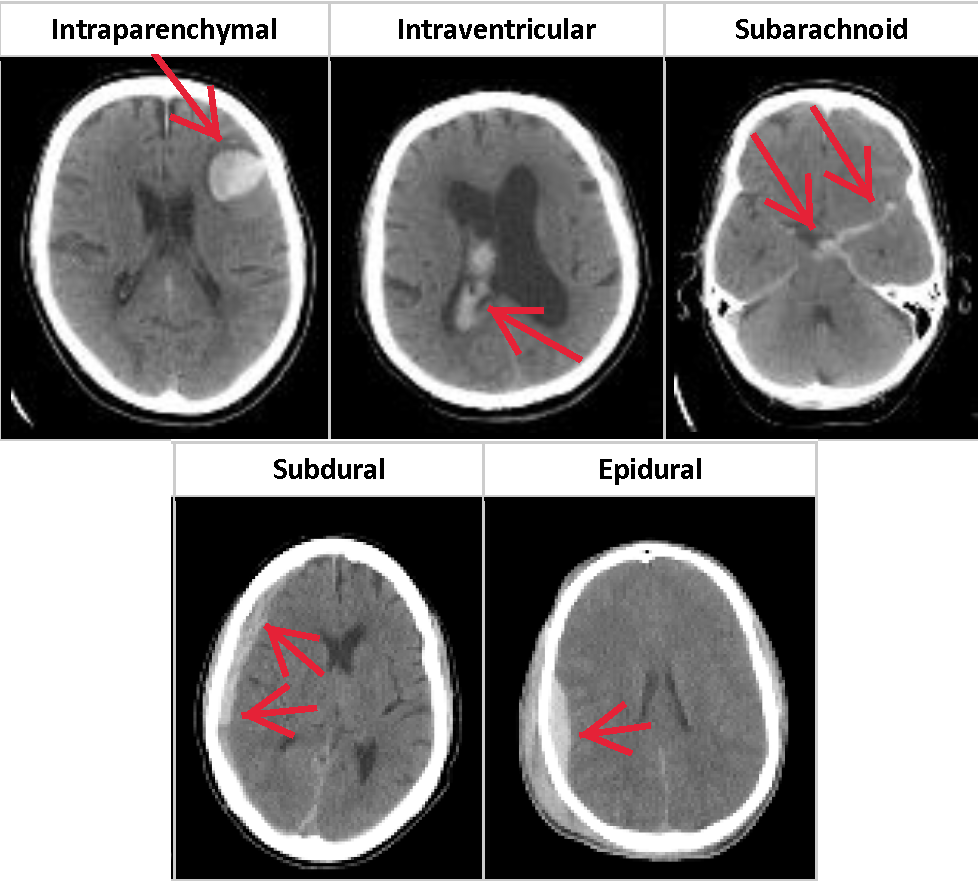
\includegraphics[scale=0.9]{images/ich-types.png}
		\centering
		\caption{CT images with different intracranial hemorrhage types. Image from \cite{kaggle_competition} (edited) (path: Overview - Hemorrhage Types)}
\end{figure}

ICH is a life-threatening condition. According to L. Januszewicz\cite{urden2019priorities}, approximately 13\,\% of strokes are hemorrhagic, and the remaining 87\,\% ischemic. Although hemorrhagic strokes are less common than ischemic, hemorrhagic strokes much more often result in death. Its mortality rate within 30 days is 37--38\,\%, where ischemic strokes cause death only in 8--12\,\% of cases.

Early and correct diagnosis is crucial for providing proper treatment. The diagnosis process consists of the patient's detailed history, if possible, physical examination, and mostly CT examination of the brain.\cite{FREEMAN2012211}
The presence of ICH is often difficult to distinguish from ischemic stroke because the symptoms are usually quite similar. However, some symptoms like headache, vomiting, neck stiffness, or coma, increase the probability of ICH compared to ischemic stroke, but only neuroimaging can provide an accurate diagnosis.\cite{CACERES2012771}

In this case, the most commonly used neuroimaging technique is a noncontrast CT. In addition to the diagnosis, various characteristics of the finding can be seen on CT images, such as its location, size, spread into the ventricular system, or the presence of edema.\cite{CACERES2012771}

\section{Computed Tomography}

Computed tomography (CT) is a medical imaging technique used in radiology. It helps to diagnose various diseases in many parts of the body, such as the brain, lungs, heart, or abdominal cavity. During the examination, the patient lies on a bed that moves slowly through the CT scanner while the rotating X-ray emits beams into the body. The X-ray detector on the opposite side of the X-ray source receives the signals and sends them to the computer. After each rotation, the computer constructs a 2D slice of the patient and after the whole process, the slices can be stacked together and form a 3D image of the examined area.\cite{nibib_ct} 

\subsection{Hounsfield Scale}
Each pixel of the CT slice represents a value on the Hounsfield scale.  This scale describes the electrodensity of the imaged tissue at a given location. The value is called the Hounsfield unit (HU) and is computed as $1000\times(\mu_{t} - \mu_{w})/\mu_{w}$, where $\mu_{t}$ is the attenuation value of the X-ray beam in a given pixel and $\mu_{w}$ is the attenuation of water.\cite{LEV2002427} Kamalian, S. et al.\cite{KAMALIAN20163} say that the typical HUs of intracranial hemorrhage are between 60–-90, but rarely they can be higher than 100. 

\begin{figure}[ht]
		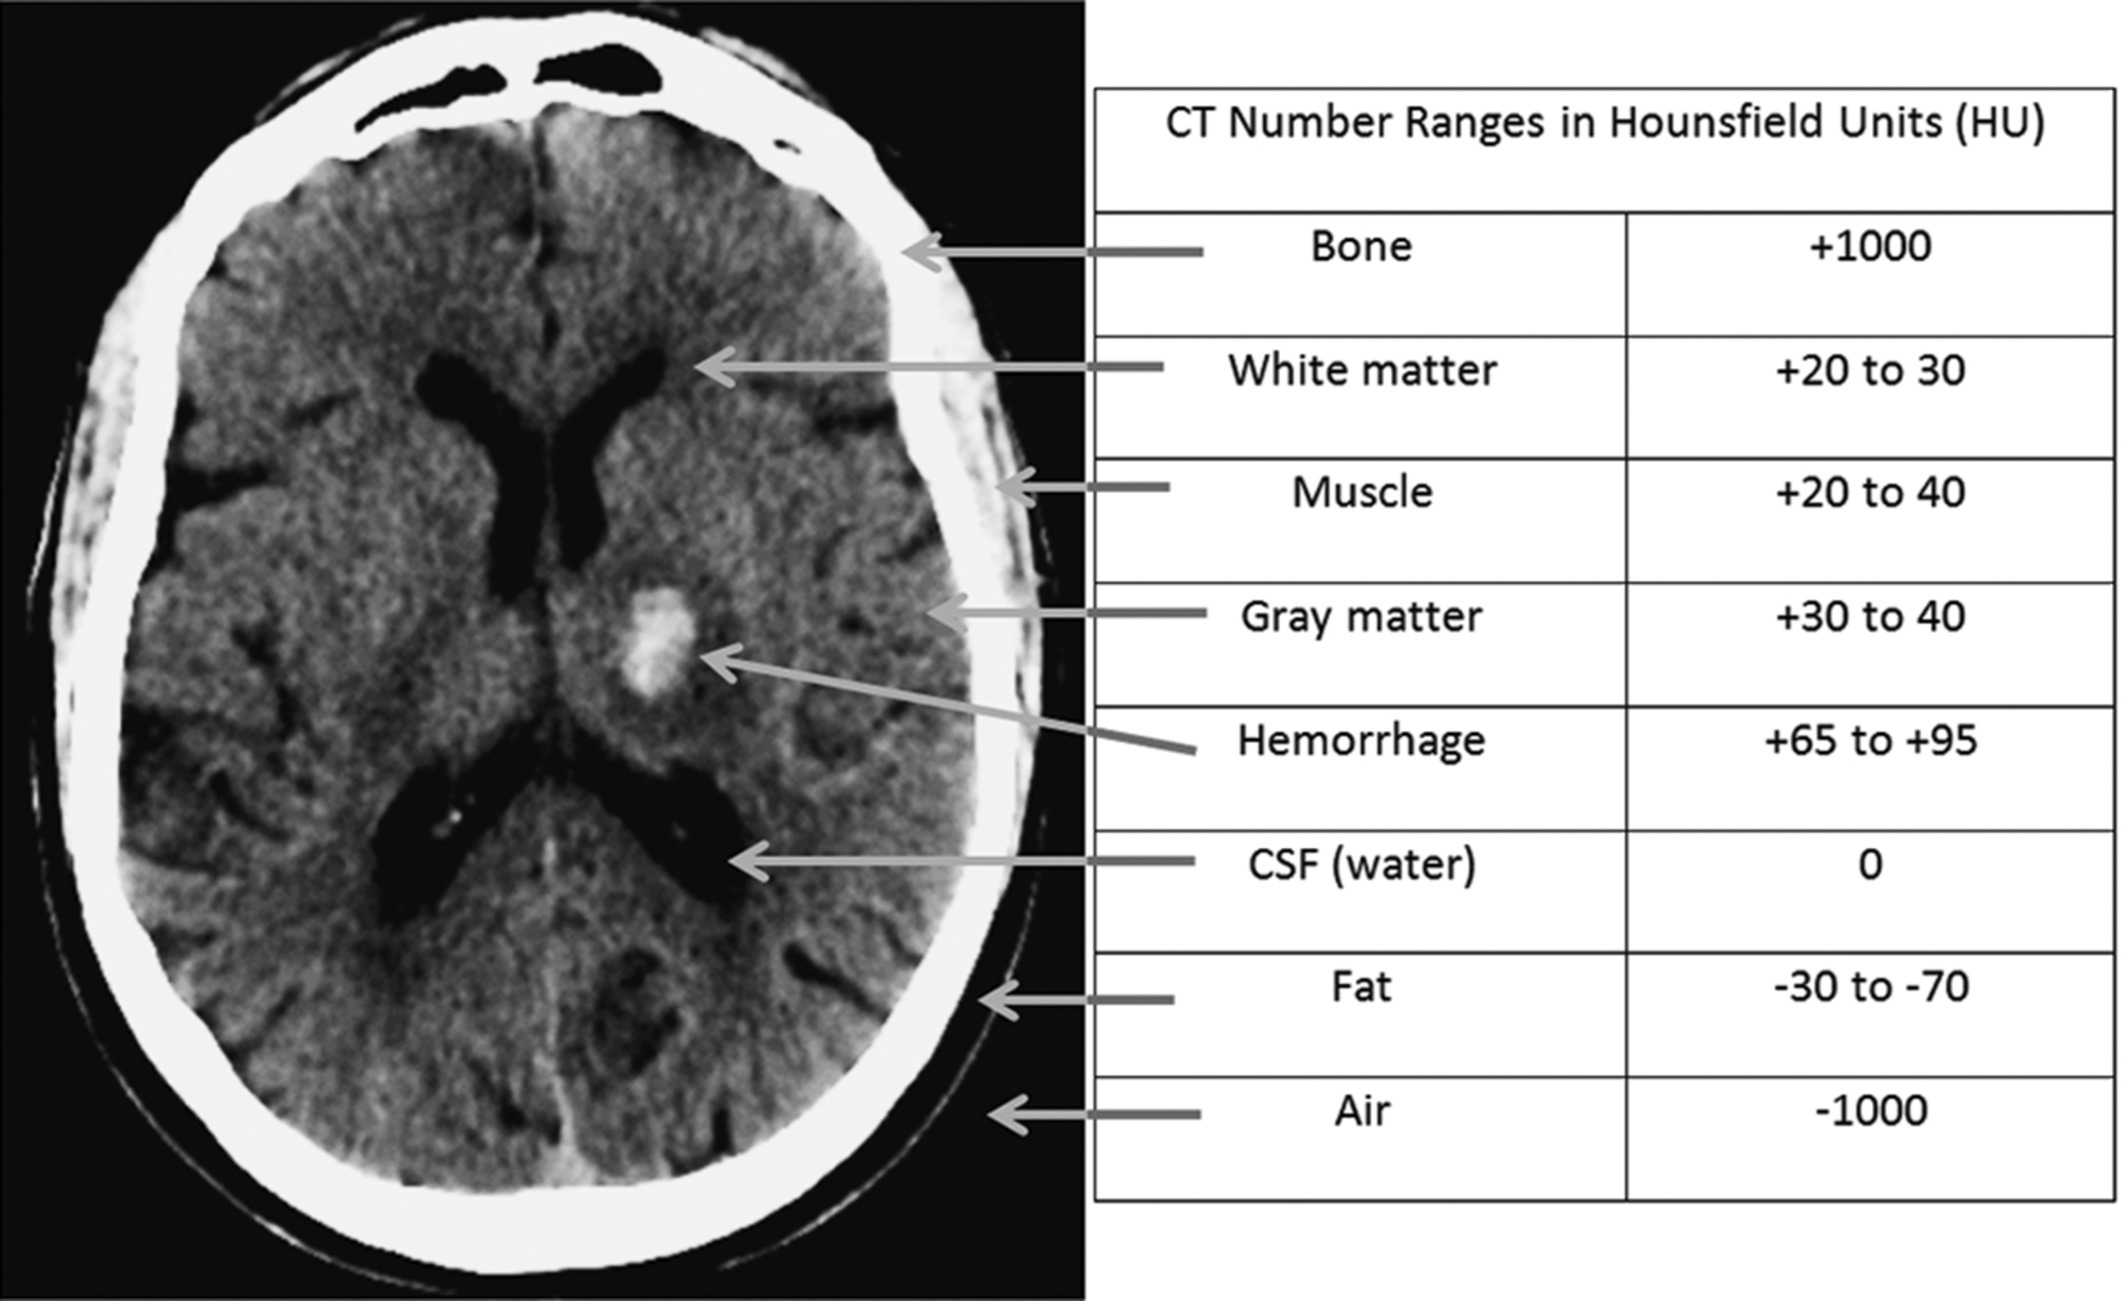
\includegraphics[scale=1.1]{images/HU-brain}
		\centering
		\caption{CT slice of a brain with examples of HU values. Image from \cite{KAMALIAN20163}.}
\end{figure}
 
The HUs range from -1000 to 1000, but the human eye can only distinguish about 128 shades of gray. Therefore the image values must be adjusted to a suitable range of HU, depending on the tissue being evaluated. The suitable range is defined by center level (CL), also called window center, and by window width (WW). The center level is the mid-value of the range, and the window width is the size of the range. Values lower than $CL - WW/2$ are black, and values greater than $CL + WW/2$ are white.\cite{KAMALIAN20163} For example, the brain window has CL 40\,HU and WW\,80 HU.\cite{murphy_windowing} It means that values lower than 0 are black and higher than 80 are white.

\begin{figure}[ht]
		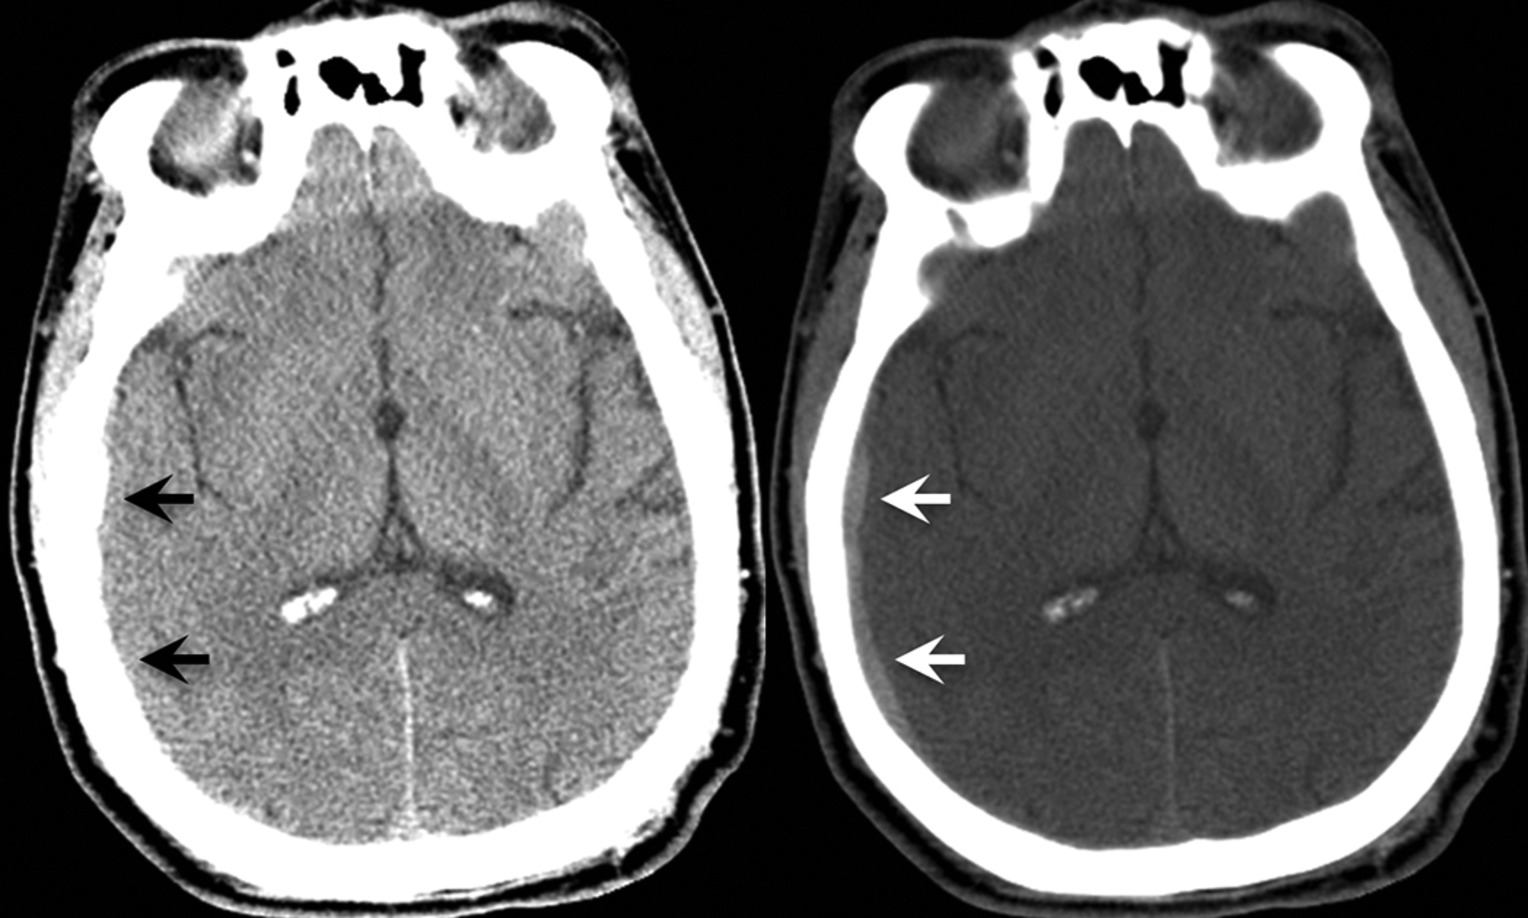
\includegraphics[scale=1.5]{images/HU-windowing}
		\centering
		\caption{CT slice with a subdural hematoma using different CL and WW. The left image has CL 30\,HU and WW 100\,HU. The right image has CL 80\,HU and WW 200\,HU. As can be seen, the hemorrhage is easier to identify with the settings in the right picture. Image from \cite{KAMALIAN20163}.}
\end{figure}

%%%%%%%%%%%%%%%%%%%%%%%%%%%%%%%%%%%%%%%%%%%%%%%%%%%%%%%%%%%%%%%%%%%%%%%%%%%%%%%%%%%%%%
%%%%%%%%%%%%%%%%%%%%%%%%%%%%%%% THEORETICAL BACKGROUND %%%%%%%%%%%%%%%%%%%%%%%%%%%%%%%
%%%%%%%%%%%%%%%%%%%%%%%%%%%%%%%%%%%%%%%%%%%%%%%%%%%%%%%%%%%%%%%%%%%%%%%%%%%%%%%%%%%%%%

\chapter{Theoretical Background}
\label{chap:theoretical_background}
This chapter provides a brief introduction to the basics of artificial neural networks. Beginning with discussing what machine learning is and then defining the most important building blocks of artificial neural networks, especially convolutional neural networks.
\section{Machine learning}
Machine learning (ML) is a subset of artificial intelligence (AI) that provides the ability of automated learning through experience and information from the given data to mathematical models. ML can be divided into two categories:

\begin{itemize}
	\item \textbf{Supervised learning}: The learning is done through labeled data. It means that the given set of data contains both the input and output values. The model is trying to learn a function that will be able to predict the output values correctly.
	\item \textbf{Unsupervised learning}: The provided data are not labeled. The goal is to learn the complex structure of the given data, find the relationships between them and divide them into clusters.
\end{itemize}

In this work, supervised learning is used. As was mentioned, the supervised learning algorithms learn to predict the label of new data as accurately as possible based on the knowledge of given labeled data. Supervised learning can also be split into two groups based on the type of labels:

\begin{itemize}
	\item \textbf{Classification}: the labels are categories;
	\item \textbf{Regression}: the labels are real numbers.
\end{itemize}

\section{Artificial Neural Networks}
An Artificial Neural Network (ANN) is a mathematical model inspired by biological neural networks. ANN consists of small interconnected units called neurons. Each input of the neuron is multiplied by its weight. These values are summed with another variable called bias. And then, the sum is passed to a nonlinear mathematical function (activation function). And based on the result, the neuron is either activated or not. The output of a neuron is used as input of another neuron or as the output of the whole network.
The formula for the output of an artificial neuron is:
\begin{equation}
    y =  \varphi \left( \sum_{i=1}^n w_{i} x_i  + b\right),
\end{equation}
where $x_i, i\in\{1, ..., n\}$ are inputs, $w_i, i\in\{1, ..., n\}$ are weights, $b$ is bias, $n$ is the number of inputs and $\varphi$ is the activation function.

\begin{figure}[ht]
		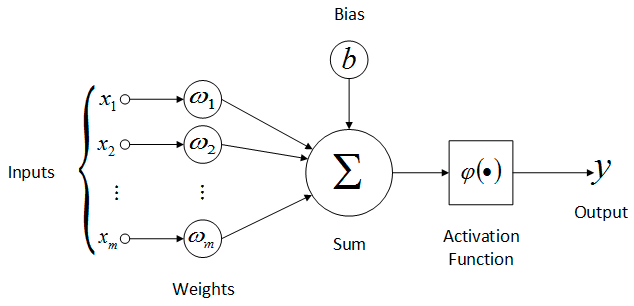
\includegraphics[scale=0.55]{images/artificial_neuron.png}
		\centering
		\caption{An artificial neuron. Image from \cite{oliveira_2017}}
\end{figure}

These neurons are then organized into layers, and the layers form an ANN. There are three basic types of layers:

\begin{itemize}
	\item \textbf{Input layer}: All inputs of each neuron in this layer are the data given to the ANN.
	\item \textbf{Output layer}: Outputs of neurons in this layer are the decisions of ANN. For example, in the case of classification, the output values are the probabilities of belonging to given classes.
	\item \textbf{Hidden layer}: Every layer between the input and output layer is a hidden layer.
\end{itemize}

The structure of an ANN can is shown in Figure \ref{fig_ann}

\begin{figure}[ht]
		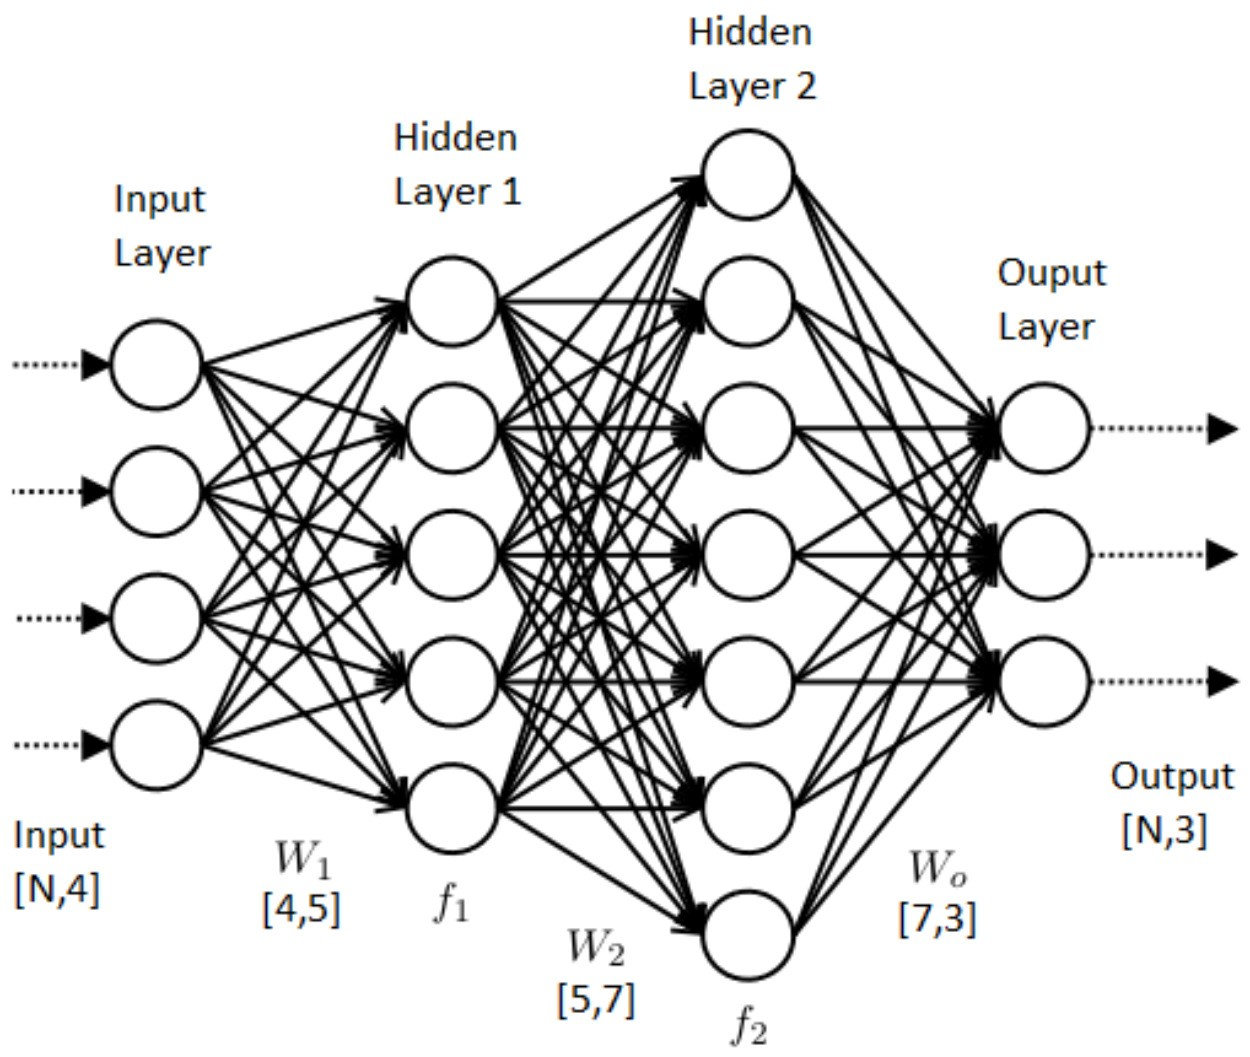
\includegraphics[scale=0.25]{images/ANN.png}
		\centering
		\caption{An ANN with two hidden layers. Image from \cite{ANN_handbook_1}}
		\label{fig_ann}
\end{figure}

\subsection{Activation functions}
Several mathematical functions can be used as activation functions. The functions must be nonlinear and differentiable. This section will discuss some of the most used ones\cite{act_fnc_2020}:

\subsubsection*{Sigmoid}
\begin{equation}
    f(x) = \frac{1}{1 + e^{-x}}
\end{equation}

\subsubsection*{ReLU}
\begin{equation}
    f(x) = \max(0, x)
\end{equation}

\subsubsection*{Leaky ReLU}
\begin{equation}
    f(x) = 
    \begin{cases}
        x & \text{if } x > 0, \\
        0.01x & \text{otherwise}.
    \end{cases}
\end{equation}

The ReLU function is the most common. It is used in hidden layers because it is more efficient than other functions like sigmoid in most cases. However, when using ReLU, sometimes the weights and biases are not updated during the learning process because the gradient can be zero. That is the reason why Leaky ReLU is used instead of ReLU in some cases. On the other hand, the sigmoid function is a common option in the output layer for classification problems due to its range which is between 0 and 1.\cite{act_fnc_2020}

\subsection{Loss functions}

The loss function is used for the computation of how well the network is performing on the given data. Usually, the goal is to minimalize the value of the loss function (loss). The choice of the function depends on the type of problem to be solved. In this section, a few loss functions for classification problems will be mentioned.

\subsubsection*{Binary cross-entropy}
One of the loss functions used when deciding in which of two classes the input belongs is binary cross-entropy (BCE) also called log loss. It can be written as follows:
$$
BCE(y, \hat{y}) = \dfrac{1}{N} \sum_{i=1}^{N} -(y_i\log(\hat{y_i}) + (1 - y_i)\log(1 - \hat{y_i}))
$$
where $y_i$ is the $i^{th}$ ground-truth label, $\hat{y_i}$ is the $i^{th}$ predicted value and $N$ is the number of predictions.

\subsubsection*{Multi-label cross-entropy}

Binary cross-entropy has to be extended in order to compute loss in multi-label classification (in multi-label classification, each sample may belongs to more than one class). For each class, the BCE is computed, and the average of these values is the multi-label cross-entropy loss.  \\

Also other loss functions can be used for classification problems, but they are not used in this work.

\subsection{Evaluation metrics}
Evaluation of the performance of an ANN model is an integral part of the implementation process. During the training, the loss function is being minimalized, but the loss does not have to be the best value for describing how accurate the model is. For further understanding of how the model performs, the different metrics are used. Note that only classification metrics are described.

The most basic metric is classification accuracy. It is the ratio of the correctly predicted values and the total number of predictions made. However, for medical problems, accuracy is an insufficient metric. The better approach is using the confusion matrix or ROC curve and AUC.

In the confusion matrix, four different values are used:

\begin{itemize}
	\item \textbf{TP (True Positives)}: the number of cases when the prediction is 1 and the label is also 1;
	\item \textbf{FP (False Positives)}: the number of cases when the prediction is 1 but the label is 0;
	\item \textbf{TN (True Negatives)}: the number of cases when the prediction is 0 and the label is also 0;
	\item \textbf{FN (False Negatives)}: the number of cases when the prediction is 0 but the label is 1.
\end{itemize}

Then the confusion matrix can be defined as shown in Figure \ref{conf_matrix}:

\begin{figure}[ht]
		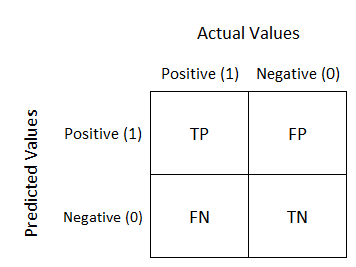
\includegraphics[scale=0.6]{images/confusion_matrix.png}
		\centering
		\caption{Confusion matrix definition. Image from \cite{confusion_matrix}}
		\label{conf_matrix}
\end{figure}

With this knowledge, the classification accuracy mentioned above can be written as:
\begin{equation}
    \dfrac{TP+TN}{TP+FP+TN+FN}
\end{equation}

In medical data classification other metrics are used:
\begin{itemize}
	\item \textbf{TPR - True Positive Rate (Sensitivity)}: 
	$$TPR = \dfrac{TP}{FN + TP}$$
	\item \textbf{FNR - False Negative Rate (Specificity)}:
	$$FNR = \dfrac{TN}{FP + TN}$$
	\item \textbf{FPR - False Positive Rate}:
	$$FPR = \dfrac{FP}{TN + FP}$$
\end{itemize}

\textbf{ROC} (receiver operating characteristics) curve is defined as a graph representing TPR and FPR at different thresholds. If the threshold is low, for example, 0.1, the model will classify all inputs whose predicted probability of being positive is higher than 0.1 as positives and lower values as negatives. That means the model will classify more inputs as positive, and the TPR and FPR will be high. On the other hand, with a higher threshold, a good model will have a lower FPR when a worse model also has a lower TPR. The ROC curve is the best way how to choose the most appropriate threshold for classification.\cite{roc_auc_google} In Figure \ref{roc} are plotted a few examples of the ROC curve.  

\textbf{AUC} (area under the ROC curve) is a metric used for measuring the model's accuracy. Its values range from 0 to 1, and the higher the value is, the better is the model.

\begin{figure}[h]
		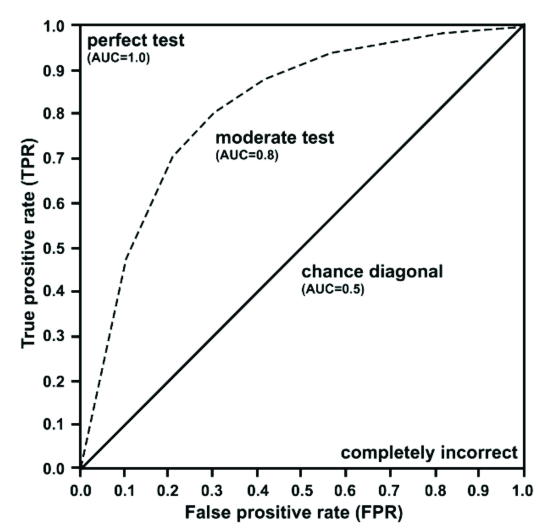
\includegraphics[scale=0.45]{images/roc_auc.png}
		\centering
		\caption{A graph with different ROC curves plotted, and their respective AUC values. Image from \cite{juliani_ellefmo_2019}}
		\label{roc}
\end{figure}

\subsection{The learning process}

The learning of an ANN is a process when the model's parameters, like weights and biases, are updated to improve the accuracy of the model. This process is called backpropagation, and it aims to minimalize the loss function.

This method requires to compute the gradient of the loss function depending on the weights and biases, according to which the weights and biases are updated, as is shown in equations below.

\begin{equation}
   W^{i+1} = W^{i} - \alpha \, \dfrac{\delta L}{\delta W^{i}} 
\end{equation}
\begin{equation}
    B^{i+1} = B^{i} - \alpha \, \dfrac{\delta L}{\delta B^{i}}
\end{equation}

where $W^{i}$ ($B^{i}$) is the vector of all the model's weights (biases) in the $i^{th}$ step, $\alpha$ is the learning rate (a value which is responsible for how big will be the learning steps of the model) and $\dfrac{\delta L}{\delta W^{i}} $ ($\dfrac{\delta L}{\delta B^{i}}$) is the gradient of loss function respective to the weights (biases) of the model.

\section{Convolutional Neural Networks}
A convolutional neural network (CNN) is a type of ANN which is broadly used for pattern recognition, mostly in image processing but also in voice recognition. The huge advantage of CNN is the low number of parameters compared to ANN.

CNNs consist of three types of layers: convolutional, pooling, and fully connected layer. In the following sections, further explanation of these layers is provided. 

\begin{figure}[ht]
		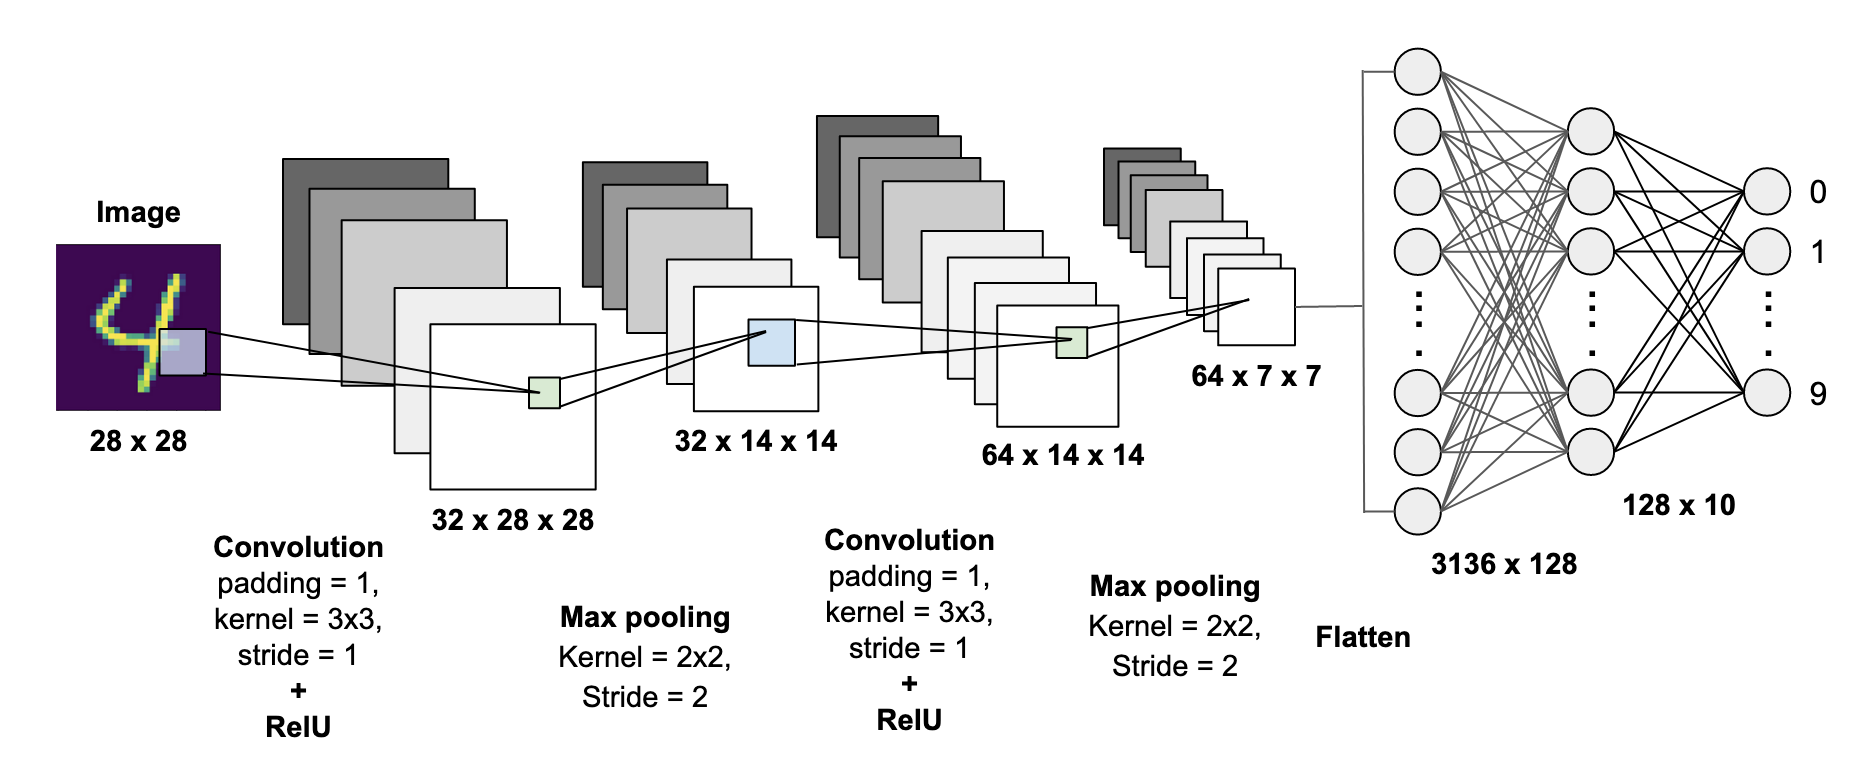
\includegraphics[scale=0.19]{images/CNN.png}
		\centering
		\caption{An example of convolutional neural network (CNN) used for digit recognition. Image from \cite{cnn_image}}
\end{figure}

\subsection{Convolutional layers}

Convolutional layers are the main building blocks of CNNs. A convolutional layer, unlike ANN's layers, does not use a weighted vector but instead of it uses an $n$-dimensional filter also called a kernel represented by a $(h\times w\times n_c)$ tensor, where $h$ is the height of the kernel, $w$ is the width, and  $n_c$ is the number of channels of the input image. The height and width may vary, but they should be odd. The most common dimensions are $3\times3$, $5\times5$, or $7\times7$. 

The convolutional layer produces its output (also called the feature map) by shifting the kernel horizontally and vertically over the input image and by computing the dot product of the kernel and image values.

\begin{figure}[ht]
		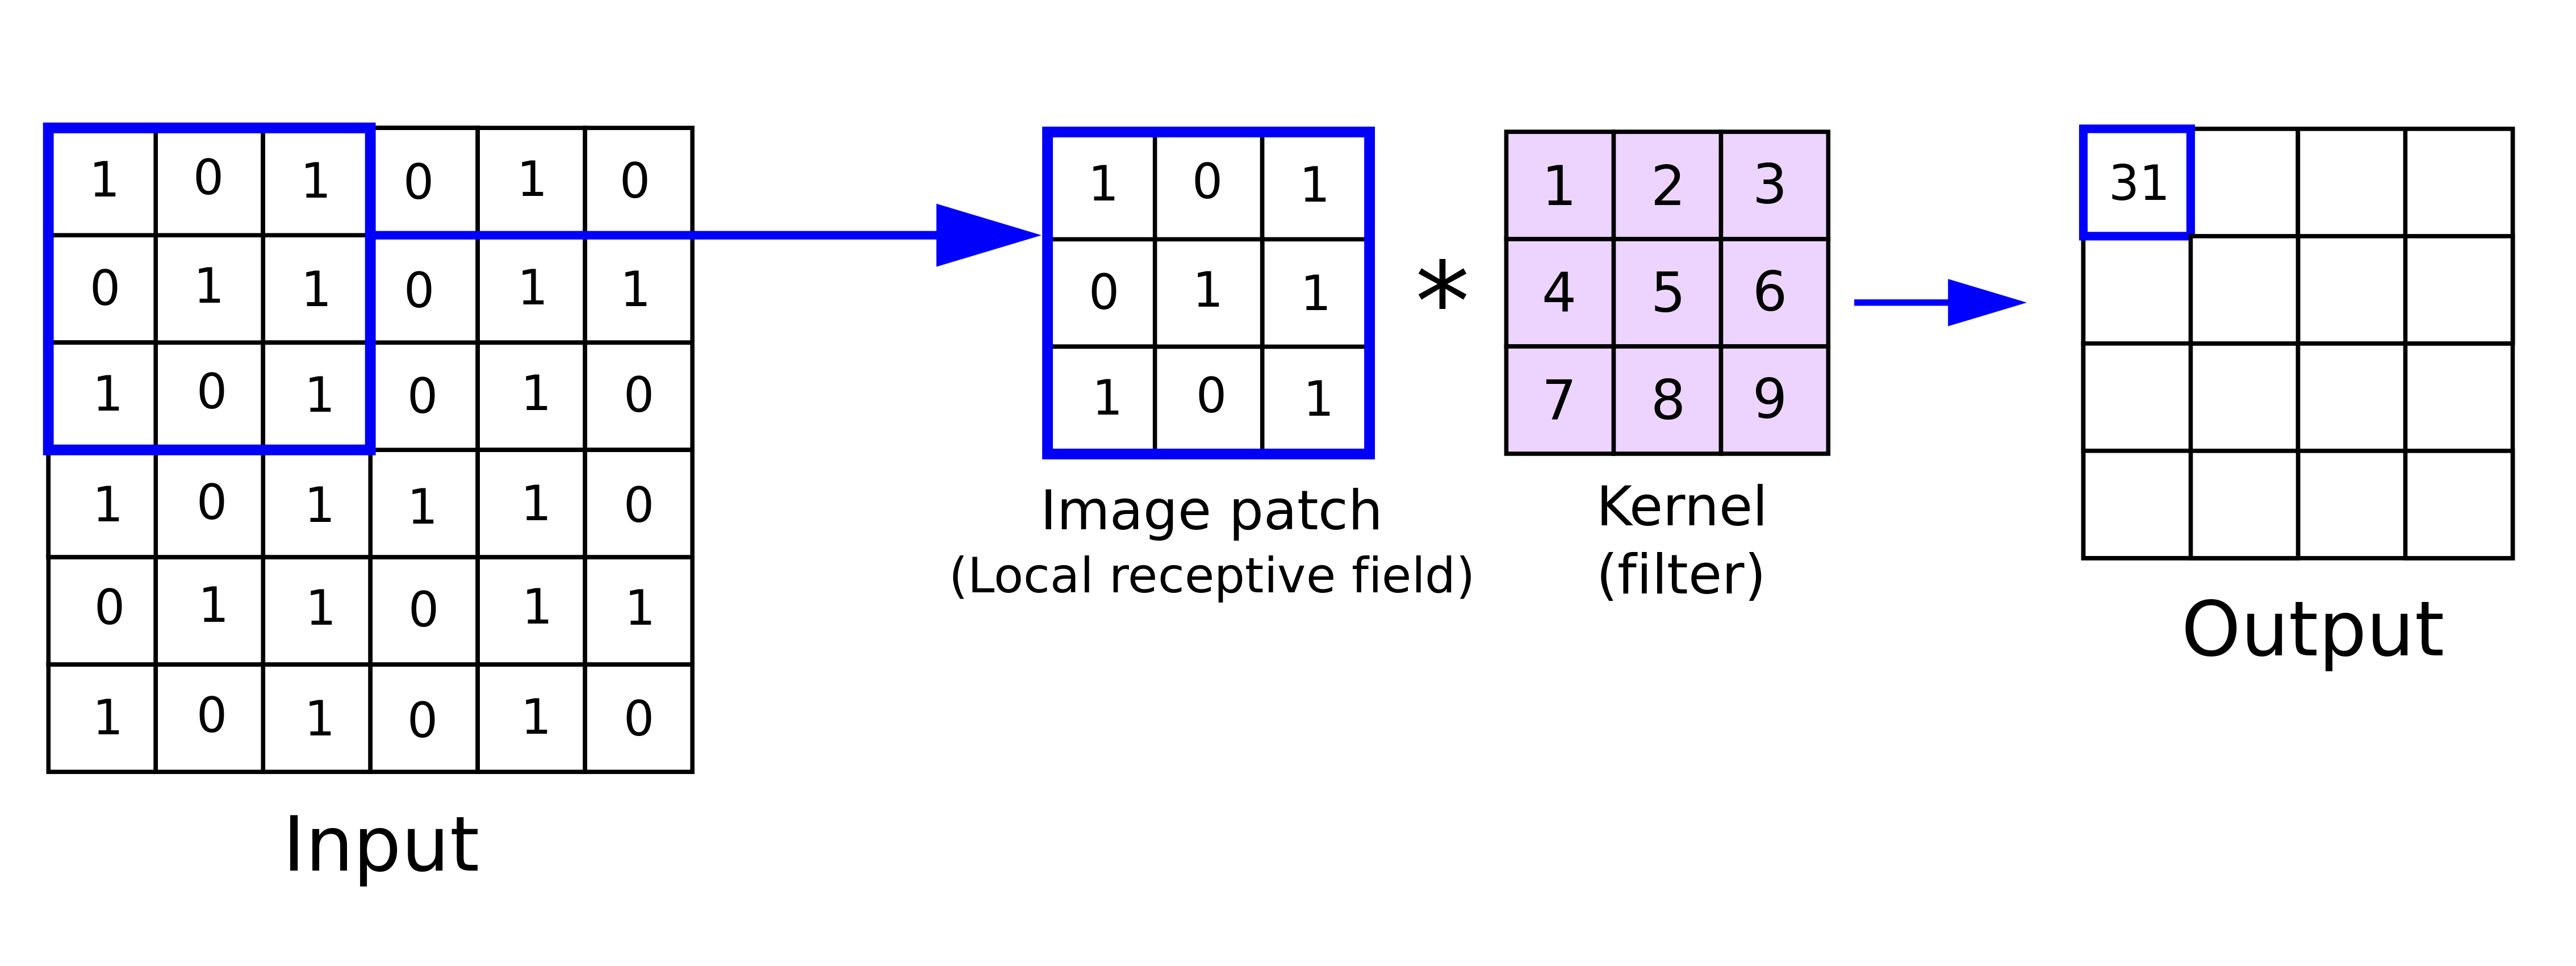
\includegraphics[scale=0.08]{images/conv_op.png}
		\centering
		\caption{Convolution using $3\times 3$ kernel. Image from \cite{convolution_op}.}
\end{figure}

In the simplest case, the dimensions of the output can be computed as $(n - f + 1, n - f + 1, n_f)$, where $n$ is the size of the input image, $f$ is the size of the filter, and $n_f$ is the number of filters used. Note that the number of kernels increases the number of channels of the output image.

However, besides the kernels count, convolutional layers have other hyperparameters:

\begin{itemize}
	\item \textbf{Padding}: Because the convolution changes the size of the input image, padding can be used if it is desired to keep the dimensions of the output image the same.
	\item \textbf{Stride}: Stride represents the step size of the kernel during the convolution. The higher the stride is, the smaller is the output image.
\end{itemize}

With the use of these hyperparameters, the size of the output image can be computed as follows:

$$
\left( \frac{n+2p+f}{s}+1, \frac{n+2p+f}{s}+1, n_f \right)
$$

where $n$ is size of the input image, $p$ is size of padding, $f$ is size of the filter, $s$ is the stride value and $n_f$ is the number of filters.

\subsection{Pooling layers}

Pooling layers are used to reduce the image size. The most commonly used type of pooling layers is max pooling and average pooling. The pooling operation is similar to convolution, but instead of convolution over the filter and the image, the max pooling takes the max value in the area and average pooling takes the average value. The pooling is applied individually on each channel, so it is preserving the number of channels. Both pooling operations, with filter size 2 and stride size 2, are shown in Figure \ref{fig:pooling}.

\begin{figure}[ht]
		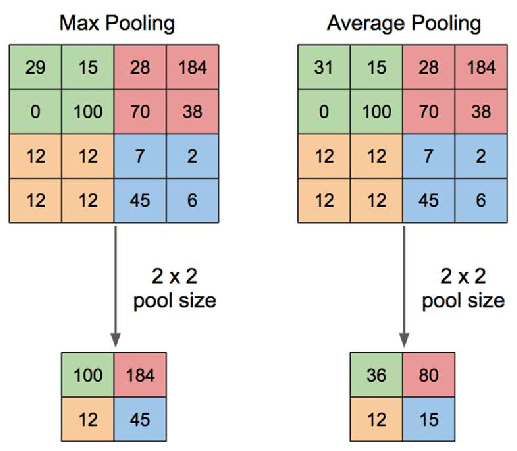
\includegraphics[scale=0.4]{images/pooling.png}
		\centering
		\caption{Schema of max pooling and average pooling. Image from \cite{yani_budhi_2019}.}
		\label{fig:pooling}
\end{figure}

\subsection{Fully connected layers}
The last type of layers used in CNN are fully connected layers (FC layers). Each neuron of the FC layer is connected to all neurons in the previous layer, like in regular ANNs. In CNN, the FC layers are used as the latest layers and serve as the final classifier.

%%%%%%%%%%%%%%%%%%%%%%%%%%%%%%%%%%%%%%%%%%%%%%%%%%%%%%%%%%%%%%%%%%%%%%%%%%%%%%%%%%%%%%
%%%%%%%%%%%%%%%%%%%%%%%%%%%%%%%%%% STATE OF THE ART %%%%%%%%%%%%%%%%%%%%%%%%%%%%%%%%%%
%%%%%%%%%%%%%%%%%%%%%%%%%%%%%%%%%%%%%%%%%%%%%%%%%%%%%%%%%%%%%%%%%%%%%%%%%%%%%%%%%%%%%%
\chapter{State of the Art}
\label{chap:state_of_the_art}
In the previous chapter, the basic building blocks of artificial and convolutional neural networks were explained. This chapter will use these basics and introduce techniques for improving the performance of neural networks and several model architectures will be described as well as some image preprocessing techniques.

\section{Image preprocessing}
In image classification tasks, preprocessing is often crucial. In many cases, it can significantly improve the performance of the model. Therefore in this section, several methods used for image preprocessing will be discussed.

\subsection{CLAHE}
A commonly used preprocessing technique for medical imaging data, especially X-ray images, is the Contrast Limited Adaptive Histogram Equalization (CLAHE). 

Histogram equalization is often used to adjust the contrast of an image. When the contrast of an image is low and the intensity values are distributed in a small interval, the histogram equalization method spreads the most frequent intensity values out of the intensity range of the image. However, this method is not really optimal, as can be seen in Figure \ref{fig:hist_eq}.

\begin{figure}[ht]
		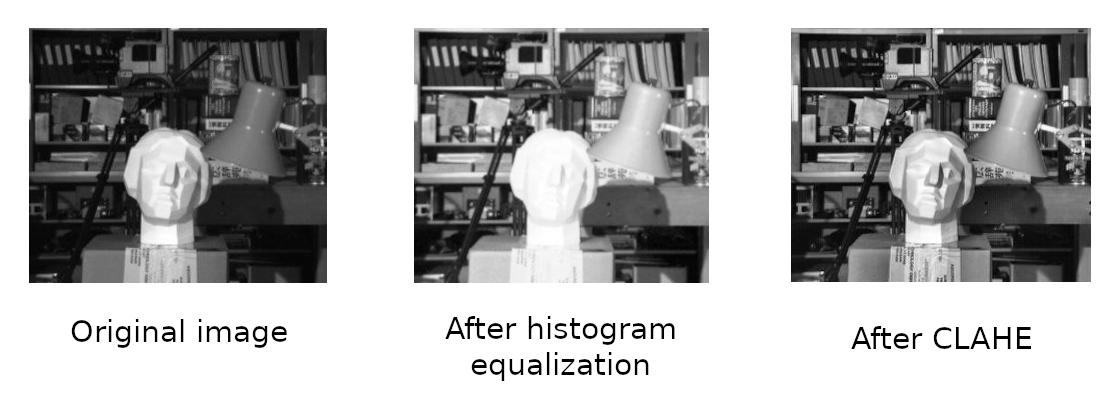
\includegraphics[scale=1.3]{images/histogram_eq.png}
		\centering
		\caption{An image (on the left) after applying histogram equalizaton (in the middle) and after using CLAHE (on the right). Images from \cite{opencv_clahe} (edited).}
		\label{fig:hist_eq}
\end{figure}

Adaptive Histogram Equalization is a modification of the histogram equalization technique. It uses multiple histograms (subhistograms) corresponding to different sections of the image in order to correct the contrast locally rather than globally. However, if there is noise in the image, it will be emphasized. To solve this problem, Adaptive Histogram Equalization with limited contrast (CLAHE) can be used. Before applying the histogram equalization, if any histogram bin is larger than a given contrast limit, these pixels are clipped and redistributed equally among all histogram bins, as shown in Figure \ref{fig:clahe}.\cite{PIZER1987355} CLAHE is often a better approach than simple histogram equalization for improving contrast in images. The comparison of these approaches is shown in Figure \ref{fig:hist_eq}.

\begin{figure}[ht]
		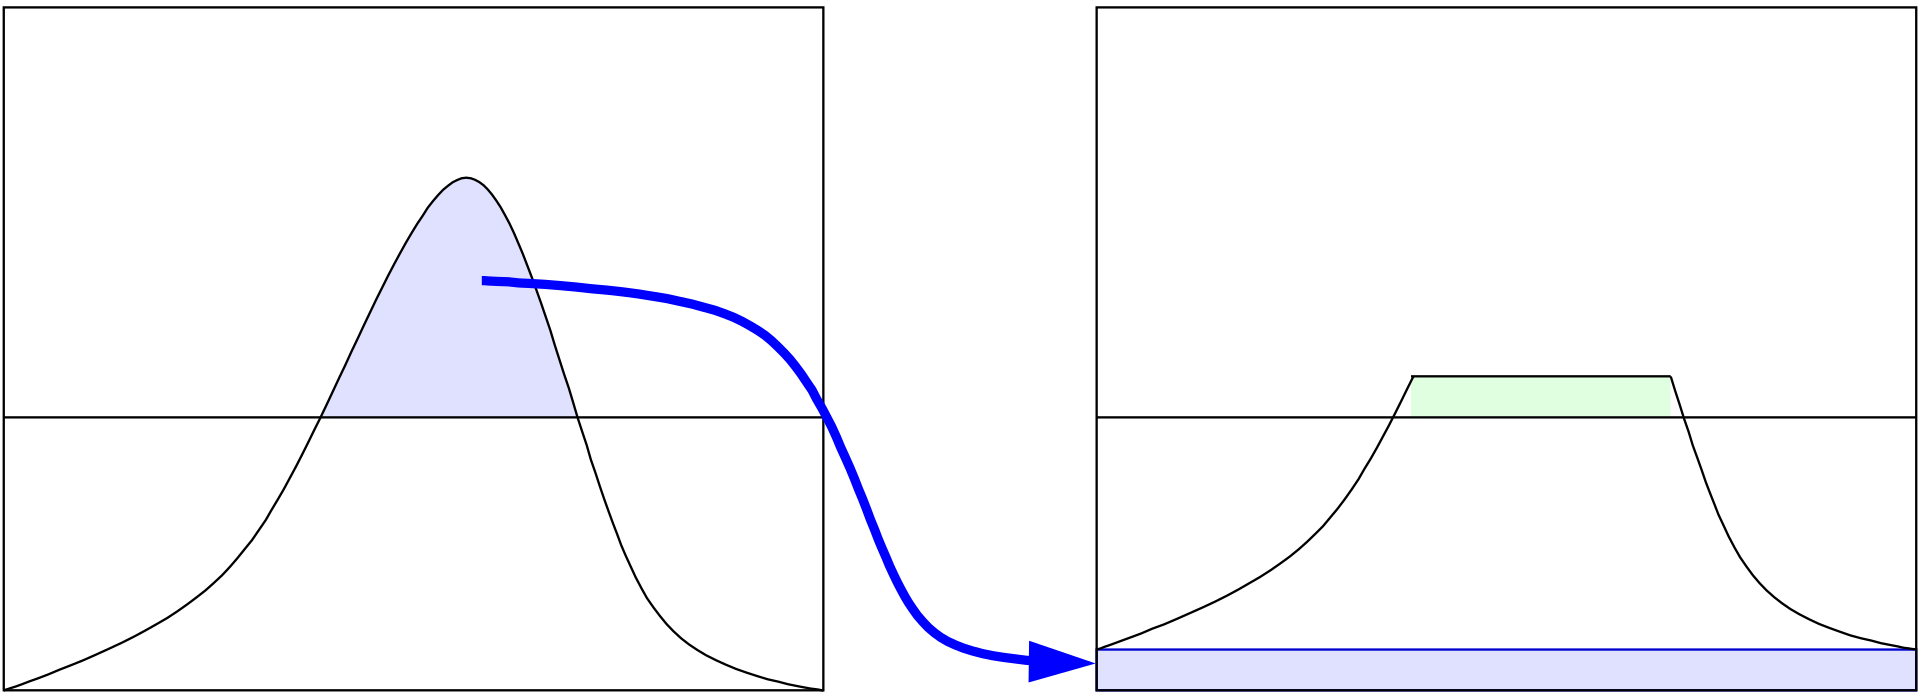
\includegraphics[scale=0.15]{images/clahe.png}
		\centering
		\caption{Redistribution of values using limited contrast. Image from \cite{wiki_ahe}.}
		\label{fig:clahe}
\end{figure}

\subsection{Image augmentation}
It is desired that a CNN performs well on test data and is able to generalize. To accomplish it, several techniques may be used (which will be discussed later), but in the image preprocessing phase, the most common method is image augmentation. 

Image augmentation creates new training data using geometric transformations, changing colors, adding noise into images, and other methods. From geometric transformations, the most used techniques are translating, rotating, flipping and zooming, but many more techniques may be used. However, it is important to preserve the same label. For example, if an image of chest X-ray is flipped, the heart will be on the right side, and this is a very rare disease, and that can affect the ground-truth label of the image.

\section{Solving underfitting and overfitting}
During training the ANN, several problems may occur. The most common are overfitting and underfitting.

\textbf{Overfitting} happens when the model learns too many details on training data and this has a negative impact on the accuracy of the test data predictions. It means that the model can fit the training data very well, but the error on test data is much higher.

There are several techniques to reduce overfitting:
\begin{itemize}
	\item increasing the number of training data, data augmentation;
	\item reducing the complexity of the model;
	\item early stopping;
	\item regularization;
	\item dropout.
\end{itemize}

The last three techniques will be explained in the following sections. \\

\textbf{Underfitting} is another problem that may happen during training the ANN. It means that the model is not able to fit neither the train data nor the test data, and both, the training error and test error are high.

To reduce underfitting, these techniques are recommended:
\begin{itemize}
	\item increasing the model complexity;
	\item increasing number of epochs.
\end{itemize}

\begin{figure}[ht]
		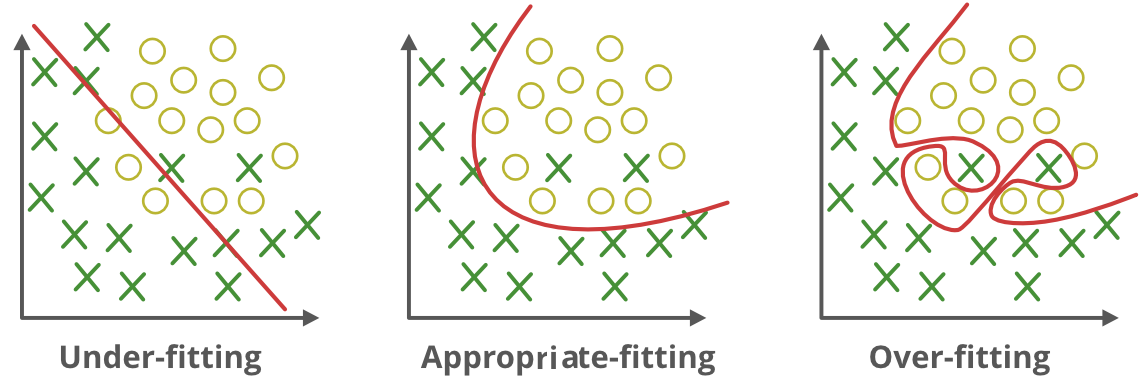
\includegraphics[scale=0.3]{images/overffiting_underfitting.png}
		\centering
		\caption{An illustration of the overfitting an underfitting problem in the classification tasks. Image from \cite{underfitting_overfitting} (edited).}
\end{figure}

\subsection{Early stopping}

While training the neural network, the training and test error should decrease monotonically with each epoch. However, at some point, the model starts overfitting and the test error begins to rise while the training error is still decreasing. Early stopping, as shown in Figure \ref{fig:early_stopping}, stops the training process right before the test error starts to increase. However, in practice is recommended to try other techniques instead of early stopping.

\begin{figure}[ht]
		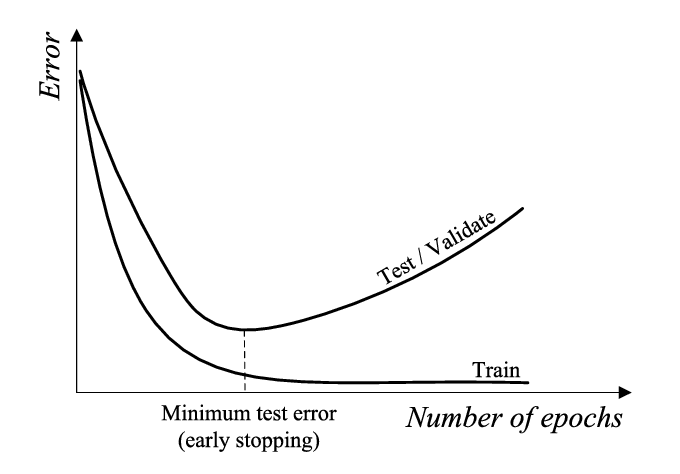
\includegraphics[scale=0.4]{images/early_stopping.png}
		\centering
		\caption{A graph of the training and the test error and the point of early stopping. Image from \cite{gencay_min_qi_2001}}
		\label{fig:early_stopping}
\end{figure}

\subsection{Regularization}

Regularization is a process of adding a penalty to the model's weights to prevent overfitting. The regularization may be written as follows:

$$L^+(W,X) = L(W,X) + \lambda R(W)$$

where $L$ is the loss function with given inputs $X$ and weights $W$, $R$ is the regularization function, and $\lambda$ is a hyperparameter that decides how much to penalize the model.

The most used regularization types are $L_1$ (lasso) regularization and $L_2$ (ridge) regularization. They are derived from the $L_1$ and $L_2$ norm of the weights' vector $w$:

$$||w||_1 = |w_1| + |w_2| + ... + |w_N|$$
$$||w||_2 = \sqrt{|w_1|^2 + |w_2|^2 + ... + |w_N|^2}$$
$$L_1 = ||w||_1$$
$$L_2 = ||w||_2^2$$

Sometimes the sum of these two types is used and is called Elastic regularization. However, the most common option is the $L_2$ regularization.\cite{Goodfellow-et-al-2016}

\subsection{Dropout}

A widely used technique is also dropout which refers to randomly \say{dropping out} some of the units. During the training phase, each unit in the network has a probability $p$ of being temporarily removed from the network. This process creates a much smaller model, and these small models are then trained. In general, when $n$ is the number of neurons in the whole network, there exist $2^n$ possible different networks derived from the original model. With each training case and another model from the $2^n$ possibilities is used.\cite{dropout_art}

Unlike regularization, the dropout can resolve a co-adaption of the network. The co-adaption is a problem when some connections within the model are significantly more powerful than others (they have the better predictive capability). It means that during training the ANN, these stronger connections learn more while the weaker connections are being ignored. Thus only a fraction of the connections is trained. However, because with every training case, different connections are trained, the ANN cannot emphasize any property, and it has to spread its weights. In this manner, the dropout prevents the network from co-adaption.\cite{dropout_art}

\begin{figure}[ht]
		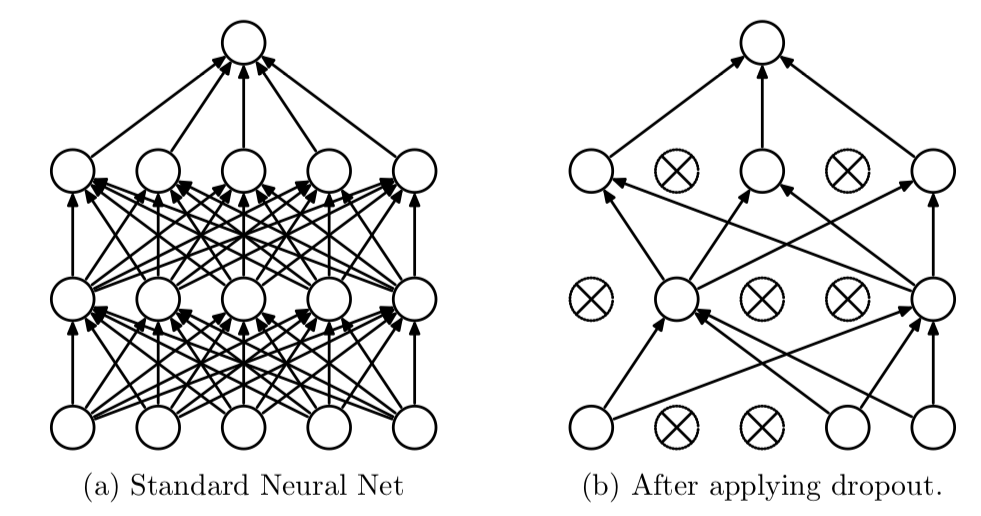
\includegraphics[scale=0.35]{images/dropout.png}
		\centering
		\caption{In the picture (a) on the left is the standard neural network, whereas in the picture (b) is the same network after applying dropout. Image from \cite{dropout_art}.}
\end{figure}


\section{Vanishing/exploding gradients}

While training a deep network, the derivatives of slopes can become very big or too small, and that makes the training problematic. During the backpropagation, while the $l$-layer neural network is trained, a total of $l$ derivatives are multiplied together. When these derivatives are large, the gradient increases exponentially, and this is the exploding gradient problem. On the other hand, when the derivatives are very small, the gradient may be nearly zero, and this is called the vanishing gradient. The problem is that the large derivatives lead to an unstable model incapable of further learning. Alternatively, if the derivatives are small, the model is not capable of learning the core features of the input data. In extreme cases, the gradient will be zero, and nothing will be learned.\cite{van_exp_gradients}

\subsection{Weights initialization}

A partial solution of the vanishing/exploding gradients may be the correct weight initialization. In order to how these weights should be initialized, Kaiming He et al. published his paper \cite{DBLP:journals/corr/HeZR015}, where he describes the correct approach of weights initialization:
\begin{itemize}
	\item The matrix of weights of each layer is initialized by values from the standard normal distribution.
	\item Each value from the matrix is multiplied by $\sqrt{2/n}$ where $n$ is the number of inputs of the particular layer.
	\item All biases are initialized by zeros.
\end{itemize}

\section{Class imbalance}
A common problem while obtaining data for neural networks training is that some classes have more samples than others. For example, this is typical for medical data because, in medical imaging, there are often significantly fewer images with some findings in them than the images without any findings. This problem is called the class imbalance problem. 

When the ANN is trained on many data with no defect and only on a few with some defect, in order to minimalize the loss function may be better to classify all the data as with no defect. The problem is that the sensitivity of a model trained on imbalanced data may be very low, and the model will not be able to recognize any finding on an image. The solution of balancing the data may be to undersample the majority class or oversample the minority, or using a combination of both is also possible. Undersampling refers to randomly deleting a certain number of samples from the majority class. On the other hand, oversampling duplicates the minority data in order to get more of them. In this case, another problem may occur because the model can start to overfit the minority classes.

Another approach is to use a weighted loss function, which gives more weight to the minority values and thus reduces the impact of the majority classes on the prediction.

\section{Patient overlap}
Another problem typical while using medical data is the patient overlap. When the data are divided into the training set and test set, the image of a patient may be in training data, while another image of the same patient is in the test set. This can lead to an overly optimistic result on the test data because the model can learn some features specific for the particular patient instead of the feature that is desired to be recognized by the model.

It has a simple solution. The dataset has to be divided into the training and test set according to patients and not according to images.

\section{Another improvement techniques}
In the previous section, some typical problems that can occur during the training of an ANN and their possible solutions were discussed. In this section, more techniques for ANN model improvement will be mentioned.

\subsection{Batch normalization}
When data from another distribution are fed into the ANN, it can negatively impact the accuracy of the model predictions. This problem is called the covariate shift. Ioffe and Szegedy published a paper \cite{DBLP:journals/corr/IoffeS15} introducing the solution to this problem - batch normalization. The solution is to normalize the inputs of individual layers. This allows training with a higher learning rate and gives more freedom in initializing the model's weights.

\subsection{Skip connections}
Deep networks are difficult to train because of the vanishing/exploding gradients. Another approach to solving this problem is using skip connections. These connections take the output of one layer and feed it into a deeper layer (as is shown in Figure \ref{fig:dropout}). This allows better propagation of the information through the ANN and the training of much deeper networks.\cite{DBLP:journals/corr/HeZRS15}

\begin{figure}[ht]
		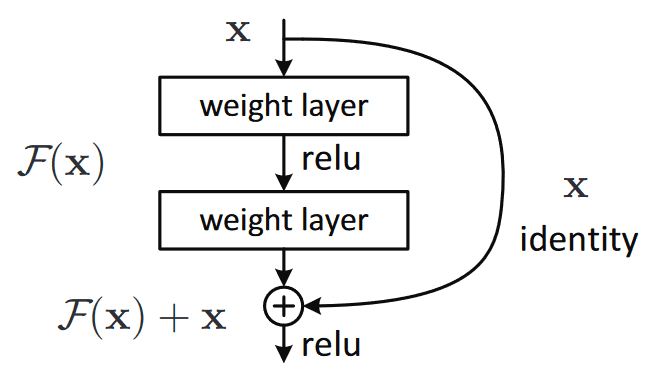
\includegraphics[scale=0.3]{images/skip_connection.png}
		\centering
		\caption{An illustration of the skip connection. Image from \cite{DBLP:journals/corr/HeZRS15}.}
		\label{fig:dropout}
\end{figure}

\subsection{Cross-validation}
Cross-validation is a widely used technique for the evaluation of the ML model's performance. The input data are divided into $d$ folds wherein each fold are $n/d$ samples where $n$ is the total number of samples. During the cross-validation, the model is trained $d$-times, where $d-1$ folds represent the training data, and the remaining one fold represents the test set. It is important that with each iteration, the test set must be a different fold. Consequently, the average of the results of the models trained in this way is more appropriate to its actual performance than the result from one training iteration.

\begin{figure}[ht]
		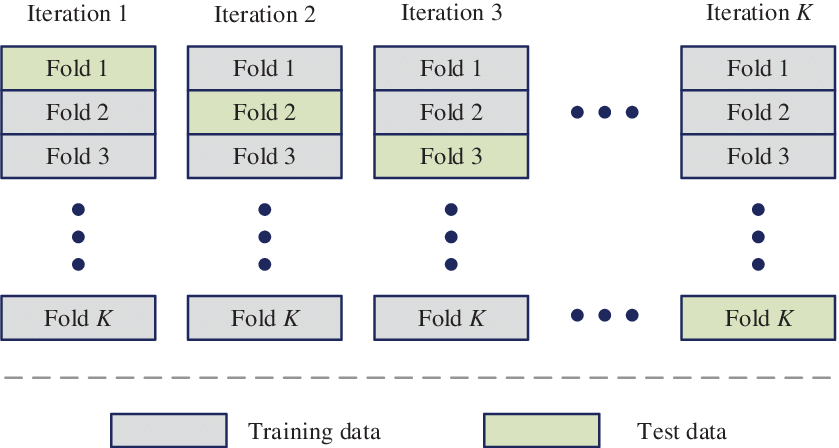
\includegraphics[scale=0.4]{images/cross_validation.png}
		\centering
		\caption{An illustration of the cross-validation with $K$ folds. Image from \cite{ren_li_han_2019}}
\end{figure}

\subsection{Transfer learning}
Training a CNN from randomly initialized weights can be time-consuming and not effective. A better approach is to use pre-trained weights from another model with the same architecture and train these weights on the new task. In the CNN model, earlier layers learn to recognize basic features like edges, and only the deeper layers recognize task-specific features. Therefore, a frequently used method of training these weights is to freeze the earlier layers and train only the parameters of the deeper layers. Another method is that the weights may be used only as initialization, and all of the network parameters are trained.

The transfer learning approach is also beneficial when there is not any large dataset available for the task.

\subsection{Model ensembling}
The model ensembling approach is that instead of one model, several slightly (or more) different models are trained, and the average prediction of individual models is taken as the final prediction. Such predictions are usually better, but one major disadvantage of this method is its time-consuming nature.

\section{CNN architectures}
A choosing the proper architecture for an ML task is one of the most crucial parts of finding the appropriate solution. Thus in this section, some of the frequently used architectures and their fundamental building blocks will be discussed.

\subsection{DenseNet}
In order to maximalize the information flow between layers in neural networks, Gao Huang et al. \cite{DBLP:journals/corr/HuangLW16a} designed a new CNN architecture called DenseNet (Dense Convolutional Network). This network consists of dense blocks separated by a convolutional and pooling layer, as shown in Figure \ref{fig:dense_net}. The dense block is like a neural network, where each layer is connected to every other layer in a feed-forward nature. It allows the network to have a relatively small number of parameters, and it improves the flow of information through the network.

\begin{figure}[ht]
		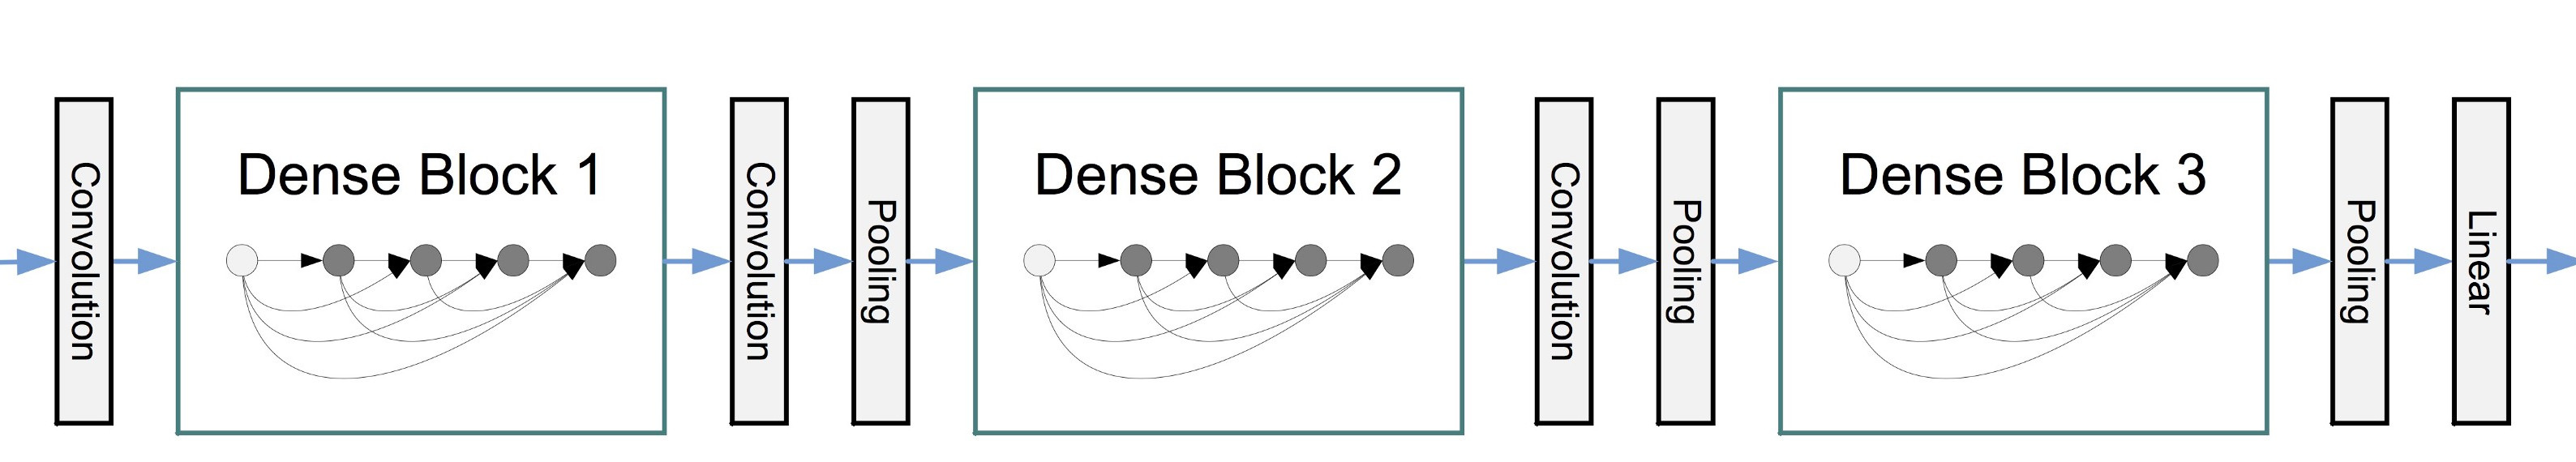
\includegraphics[scale=0.115]{images/DenseNet.jpeg}
		\centering
		\caption{The DenseNet architecture with three dense blocks. Image from \cite{DBLP:journals/corr/HuangLW16a} (edited).}
		\label{fig:dense_net}
\end{figure}

\begin{figure}[ht]
		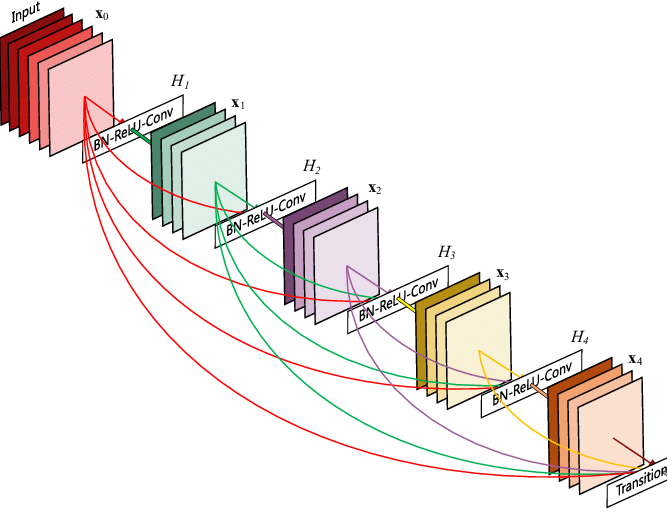
\includegraphics[scale=0.4]{images/dense_block.png}
		\centering
		\caption{The dense block with five layers. Image from \cite{DBLP:journals/corr/HuangLW16a}.}
\end{figure}

\subsection{ResNet}
In the past, training very deep neural networks were impossible because of the vanishing/exploding gradients problem, which was partly solved by input normalization and batch normalization. However, while increasing the number of layers, at some point, the training and test error also start to increase. This problem was solved by Kaiming He et al. by introducing the skip (shortcut) connections and Residual Networks \cite{DBLP:journals/corr/HeZRS15}. The baseline of the residual network is a simple CNN. The difference is that the ResNets add skip connections into the network, as shown in Figure \ref{fig:res_net}. This makes possible to train deep neural networks more efficiently and with better performance.

\begin{figure}[ht]
		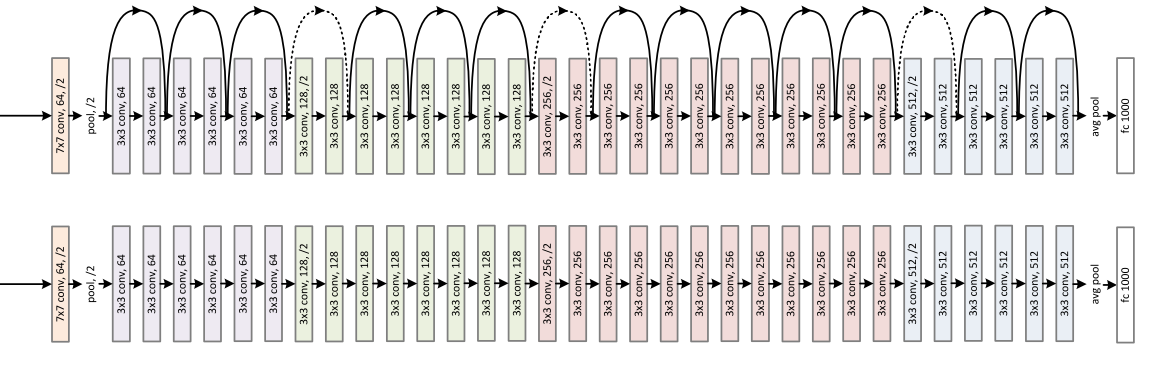
\includegraphics[scale=0.32]{images/ResNet.png}
		\centering
		\caption{And example of a plain architecture (on the bottom) and ResNet architecture (on the top). Image from \cite{DBLP:journals/corr/HeZRS15} (edited).}
		\label{fig:res_net}
\end{figure}

\subsection{EfficientNet}
Mingxing Tan and Quoc V. Le \cite{DBLP:journals/corr/abs-1905-11946} have studied the effect of scaling the neural network on its accuracy and efficiency. During their research, they developed a new type of models called EfficientNets, which had a much better performance, according to number of parameters, than the other convolutional networks they tried, such as DenseNet, ResNet, Inception and others. The EfficientNet architecture mainly consists of a mobile inverted bottleneck convolution (MBConv) block built of inverted residuals with linear bottlenecks.

Usually, a skip connection in residual blocks connects the wider layers. Between the connected layers by the skip connection, the number of channels of the input is reduced and then increased, as shown in Figure \ref{fig:res_block} on the top. When this block is inverted, the skip connection connects the more narrow layers, and between these layers, the input increases its number of channels and then decreases, as shown in Figure \ref{fig:res_block} on the bottom.\cite{DBLP:journals/corr/abs-1801-04381}

\begin{figure}[ht]
		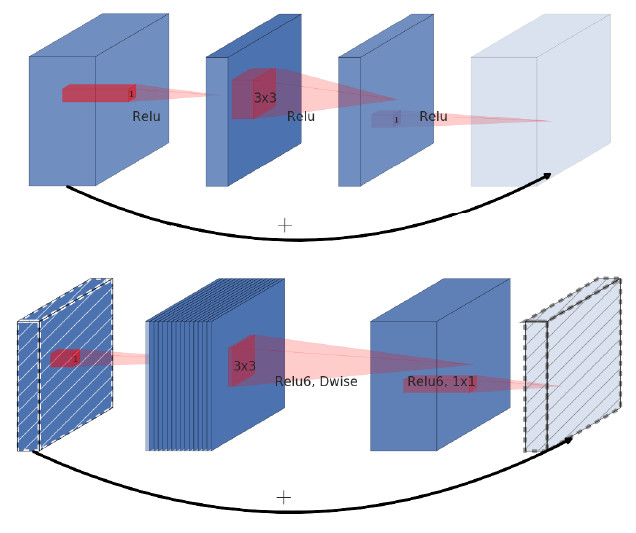
\includegraphics[scale=0.5]{images/res_block_and_inv_res_block.jpeg}
		\centering
		\caption{On the top: the residual block, on the bottom: the inverted residual block. Image from \cite{DBLP:journals/corr/abs-1801-04381} (edited).}
		\label{fig:res_block}
\end{figure}

The linear bottleneck means that the last convolutional operation of the inverted residual block has only a linear output instead of using the ReLU activation. Because the ReLU causes some loss of information (when the values are lower than zero) as well as decreasing the number of channels that happens in the last layer of the residual block.\cite{DBLP:journals/corr/abs-1801-04381}

\subsection{Inception Networks}
In image recognition and classification problems, the main features of the image often vary in size. Hence, sometimes is difficult to choose the proper size of the convolutional filter because when the main feature is more spread or larger, a filter of a bigger size can process the information more effectively, and when the main feature is smaller, then it is better to use a smaller filter size. Therefore, Christian Szegedy et al. \cite{DBLP:journals/corr/SzegedyLJSRAEVR14} come with a solution using networks with Inception modules.

In its most naive version, the inception module consists of three convolution operations and one max pooling operation performed over the same input. Results are then concatenated into the module output. Because computing three times more convolutions is computationally expensive, a new inception module with dimensional reduction was introduced. This reduction is made by $1\times1$ convolutions because this convolutional operation persists the width and height of the input, and it can decrease the number of channels. %The scheme of these modules is shown in Figure \ref{fig:inc_block}.\cite{DBLP:journals/corr/SzegedyLJSRAEVR14}

%\begin{figure}[ht]
%		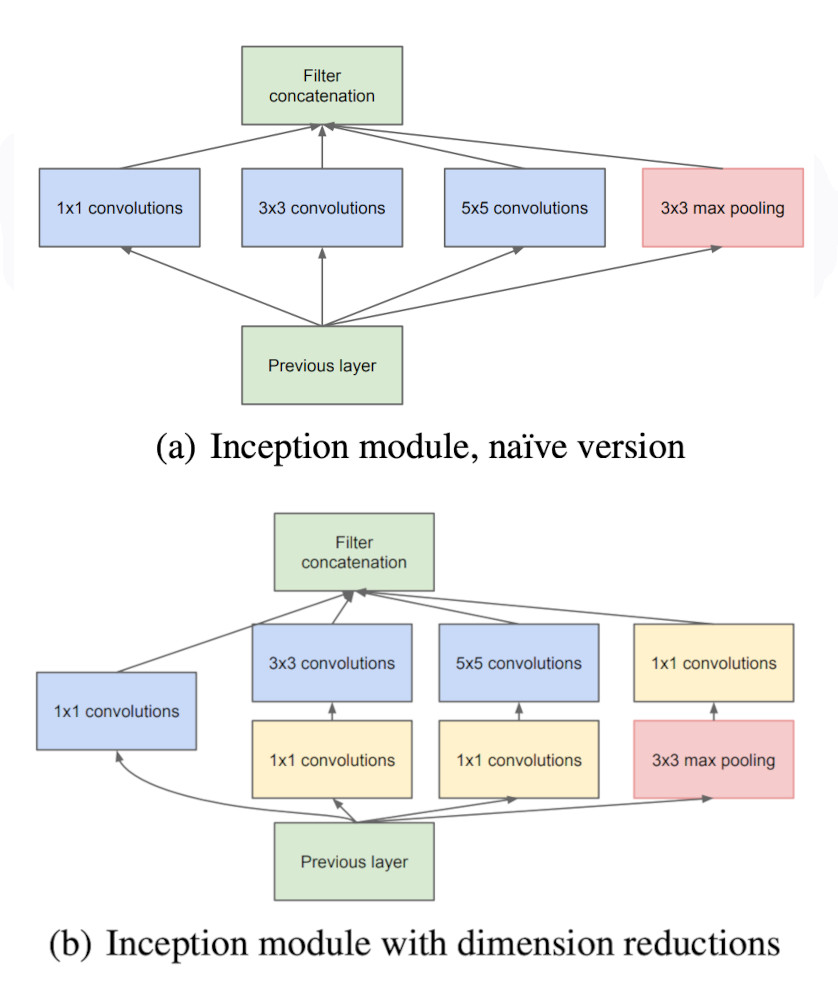
\includegraphics[scale=0.3]{images/inception_blocks.jpeg}
%		\centering
%		\caption{The naive version of the inception module (a) and the version with dimension reductions (b). Image from \cite{DBLP:journals/corr/SzegedyLJSRAEVR14} (edited).}
%		\label{fig:inc_block}
%\end{figure}
%
Using the inception modules with dimensional reduction, the Inception v1 architecture was constructed (also known as GoogLeNet). It is the simplest version of the Inception Network.\cite{DBLP:journals/corr/SzegedyLJSRAEVR14} There are several upgraded versions (Inception v2, v3, v4, and others), but the main principle is similar. 

%%%%%%%%%%%%%%%%%%%%%%%%%%%%%%%%%%%%%%%%%%%%%%%%%%%%%%%%%%%%%%%%%%%%%%%%%%%%%%%%%%%%%%
%%%%%%%%%%%%%%%%%%%%%%%%%%%%%%%%%% RELATED STUDIES %%%%%%%%%%%%%%%%%%%%%%%%%%%%%%%%%%%
%%%%%%%%%%%%%%%%%%%%%%%%%%%%%%%%%%%%%%%%%%%%%%%%%%%%%%%%%%%%%%%%%%%%%%%%%%%%%%%%%%%%%%

\chapter{Related studies}
\label{chap:related_studies}
It is not the first time when is desired to detect intracranial hemorrhages using artificial neural networks. Many studies have been published in order to develop an accurate algorithm. Thus in this chapter, several studies and approaches that aimed to solve this task will be discussed.

In 2018, Srivastava et al. \cite{DBLP:1710-04934} implemented their own architecture called RADnet, a combination of DenseNet and Long Short Term Memory (LSTM) network. They used 40-layer DenseNet with three auxiliary tasks to segment the hemorrhagic regions. This approach allows the network to focus on relevant features, which improves the model's performance. Also, to incorporate the context from the neighboring slices, the LSTM network was added to the model. 

LSTM is a recurrent neural network (RNN) architecture. RNNs are able to learn patterns from variable length sequence inputs. They are mostly used in natural language processing. However, they can also be used for CT images because the whole CT scan consists of a sequence of slices. The standard RNN has a loop over the hidden unit, as shown in Figure \ref{fig:rnn}, where is also illustrated the unfolded version, which is equivalent to the folded version, and it is basically repeating the same structure multiple times.\cite{feng_guan_li_zhang_luo_2017}
\begin{figure}[ht]
		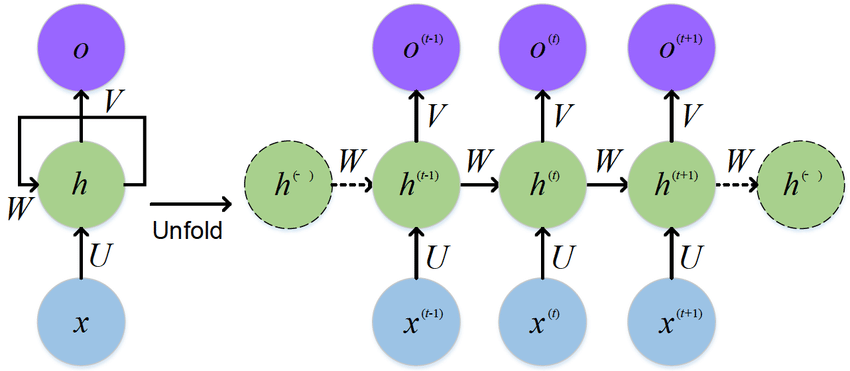
\includegraphics[scale=0.3]{images/rnn.png}
		\centering
		\caption{The standard folded (on the left) and unfolded (on the right) RNN. Image from \cite{feng_guan_li_zhang_luo_2017}.}
		\label{fig:rnn}
\end{figure}

The LSTM differs from standard RNN by the structure of the hidden layer. In standard RNN, the output $y$  at time $t$ is computed from the hidden layer $h$ as:
\begin{align*}
    h_{(t)} & = \sigma(Ux_{(t)}+Wh_{(t-1)}+b)\\
    y_{(t)} & = \sigma(Vh_{(t)}+c)
\end{align*}
where $x$ is the input, $b$ and $c$ are bias vectors, $U$, $V$, and $W$ are the weight matrices, and $\sigma$ is the sigmoid function.\cite{yuan_li_wang_2020}

In the LSTM network, the output at time $t$ is calculated as:
\begin{align*}
    f_{(t)} & = \sigma(W_{fx}x_{(t)}+W_{fh}h_{(t-1)}+b_{f})\\
    i_{(t)} & = \sigma(W_{ix}x_{(t)}+W_{ih}h_{(t-1)}+b_{i})\\
    o_{(t)} & = \sigma(W_{ox}x_{(t)}+W_{oh}h_{(t-1)}+b_{o})\\
    C_{(t)} & = \tanh(W_{cx}x_{(t)}+W_{ch}h_{(t-1)}+b_{c})\\
    c_{(t)} & = f_{(t)} \odot C_{(t)} + i_{(t)} \odot C_{(t)}\\
    h_{(t)} & = o_{(t)} \odot \tanh(c_{(t)})
\end{align*}

where function $f$ is called forget gate, $i$ input gate and $o$ output gate, $x$ is the input, $b_{f}$, $b_{i}$, $b_{o}$ and $b_{c}$ are bias vectors, $W_{:x}$ and $W_{:h}$ are the weight matrices, $\sigma$ is the sigmoid function and the function $c$ is called cell state and $h$ is the hidden state.\cite{yuan_li_wang_2020} The visualization of LSTM unit is shown in Figure \ref{fig:lstm}.
\begin{figure}[ht]
		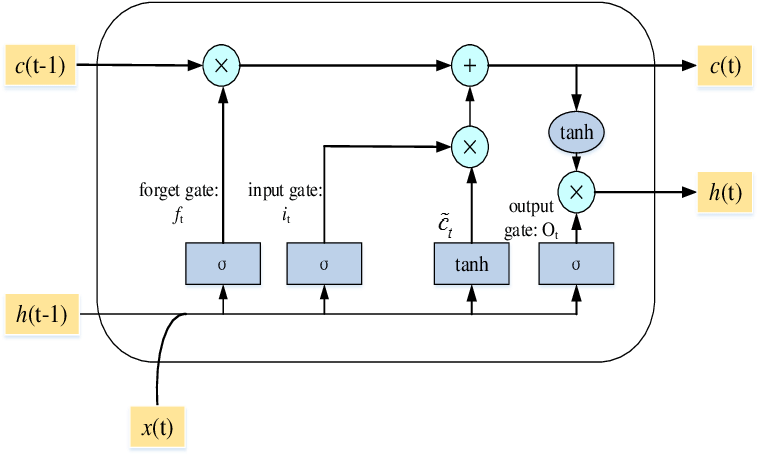
\includegraphics[scale=0.4]{images/lstm.png}
		\centering
		\caption{The structure of the LSTM unit. Image from \cite{yuan_li_wang_2020}.}
		\label{fig:lstm}
\end{figure}

This implementation performed very well (81.82\% hemorrhage prediction accuracy) and was comparable to the predictions of three senior radiologists.

Weicheng Kuo et al. (2019) \cite{Kuo22737} used another approach. They build their solution on Dilated ResNet (DRN). The DRN was introduced by Fisher Yu et al. \cite{DBLP:journals/corr/YuKF17}. It is a modified ResNet architecture that does not reduce the image resolution to small feature maps, but it preserves the resolution. The intuition behind this approach is that by reducing the spatial dimensions of the input image, some important small features may be suppressed. Moreover, because of that, the model cannot further improve its accuracy. In ResNets, the downsampling of the input image is done by striding, so the first idea is to eliminate the striding from some layers. However, this reduces the receptive field of deeper layers, and it has a negative impact on the performance of the model. In order to preserve the perceptive field and context information, instead of simple convolutions, the dilated convolutions are used. Dilated convolution is computed similarly to regular convolution, but it uses different pixels of the image to preserve the receptive field, as shown in Figure \ref{fig:dilation}. The size of the field is defined by the dilation factor. When in one of the ResNet layers, the input is spatially reduced by a stride of two, the dilation factor will also be two. However, if in another layer, the input is again reduced by two, the dilation factor will be four in order to preserve the contextual information. The impact of the dilation factor on the convolution is illustrated in Figure \ref{fig:dilation}.

\begin{figure}[ht]
		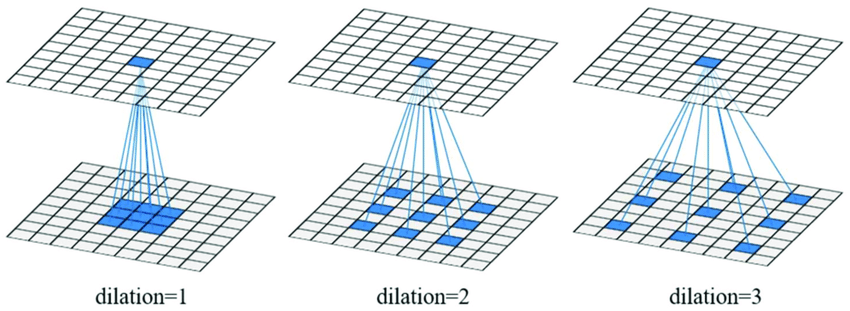
\includegraphics[scale=0.4]{images/dilation.png}
		\centering
		\caption{An illustration of the dilation convolution with different dilation factors. Note that the dilation convolution with the factor 1 (on the left) is equal to the regular convolution. Image from \cite{cui_zheng_gao_zhang_yang_ren_2019}.}
		\label{fig:dilation}
\end{figure}


This model achieved the area under the curve (AUC) of 0.991 ± 0.006, which is also very satisfying.

Another approach was implemented by P.D. Chang et al. \cite{Chang1609}. Their model was trained on more than 512 000 images from CT scans, and the solution was based on custom hybrid 3D/2D architecture derived from Region with Convolutional Neural Network (R-CNN). R-CNN architecture is used for image segmentation. It is based on a method that generates 2000 regions from the input image. Each of these regions is fed into a pretrained CNN. The feature maps obtained from the CNN are then classified, and the bounding boxes of the objects are computed.\cite{DBLP:journals/corr/GirshickDDM13}

\begin{figure}[ht]
		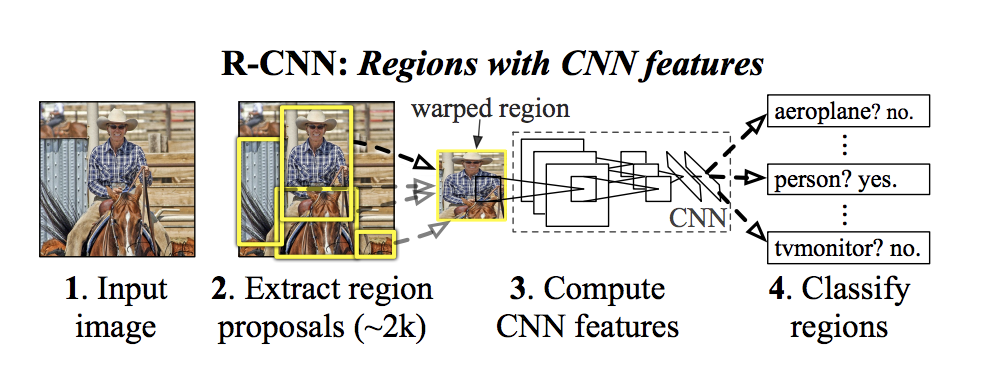
\includegraphics[scale=0.3]{images/rcnn.png}
		\centering
		\caption{The scheme of R-CNN architecture. Image from \cite{DBLP:journals/corr/GirshickDDM13}.}
\end{figure}

With this algorithm, they achieved excellent results. The accuracy, AUC, sensitivity, and specificity of the model were 0.970, 0.981, 0.951, and 0.973 on the test set.

The last study, which will be mentioned in this work, was done by Junghwan Cho et al. In their paper \cite{Cho2019}, they presented a cascaded model consisting of two convolutional neural networks (CNNs) for classification and two fully convolutional networks (FCNs) for the hemorrhage segmentation. The architecture of FCNs is similar to regular CNNs but the fully connected layers are replaced by $1 \times 1$ convolution. Thus the output is not a single label but an image smaller than the input image from which is computed the segmentation mask.\cite{DBLP:journals/corr/ShelhamerLD16}

In their cascaded model, each sample was fed into the first CNN, and if the sample was classified as positive, it was sent to the two FCNs. Otherwise, if the sample was classified as negative, it was classified again by the second CNN. This CNN reviews the sample if it is truly negative. If there is some hemorrhage detected, it is sent to the FCNs. The result from the FCNs is a segmentation map that is created by merging the two segmentation maps obtained from both FCNs. 

With this architecture, their results were great with sensitivity (97.91\% [± 0.47]) and specificity (98.76\% [± 0.10]). 

%%%%%%%%%%%%%%%%%%%%%%%%%%%%%%%%%%%%%%%%%%%%%%%%%%%%%%%%%%%%%%%%%%%%%%%%%%%%%%%%%%%%%%
%%%%%%%%%%%%%%%%%%%%%%%%%%%%%%%%%%%% REALIZATION %%%%%%%%%%%%%%%%%%%%%%%%%%%%%%%%%%%%%
%%%%%%%%%%%%%%%%%%%%%%%%%%%%%%%%%%%%%%%%%%%%%%%%%%%%%%%%%%%%%%%%%%%%%%%%%%%%%%%%%%%%%%

\chapter{Realization}
\label{chap:realization}
\section{Dataset}
The dataset used for this task was taken from the RSNA Intracranial Hemorrhage Detection competition. The aim of this competition is to develop an algorithm that will be able to classify intracranial hemorrhage subtypes in a head CT slice accurately. It consists of 752\,804 CT slices from a total of 21\,744 studies. Each slice is labeled with six labels - five corresponding to the hemorrhage types and one label \say{any}, indicating if any ICH type is present on the given slice. Also, there are other 121\,233 non-labeled slices intended for the evaluation of the competition.

\begin{figure}[ht]
		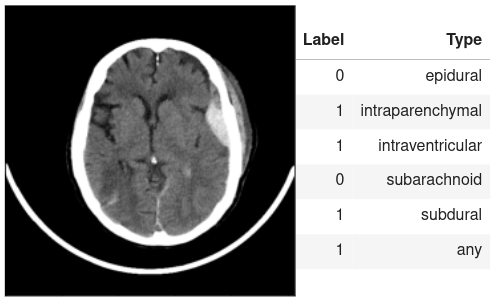
\includegraphics[scale=2.1]{images/dataset_sample.png}
		\centering
		\caption{A sample from the dataset with labels.}
\end{figure}

The training dataset contains  644\,874 images with no hemorrhage detected and 107\,933 studies with detected intracranial hemorrhage. In one image, more than one ICH type can be present. The ratio between the number of hemorrhage types is shown in Figure \ref{fig:types_ratio}. According to the graphs, the dataset is highly imbalanced.

\begin{figure}[ht]
		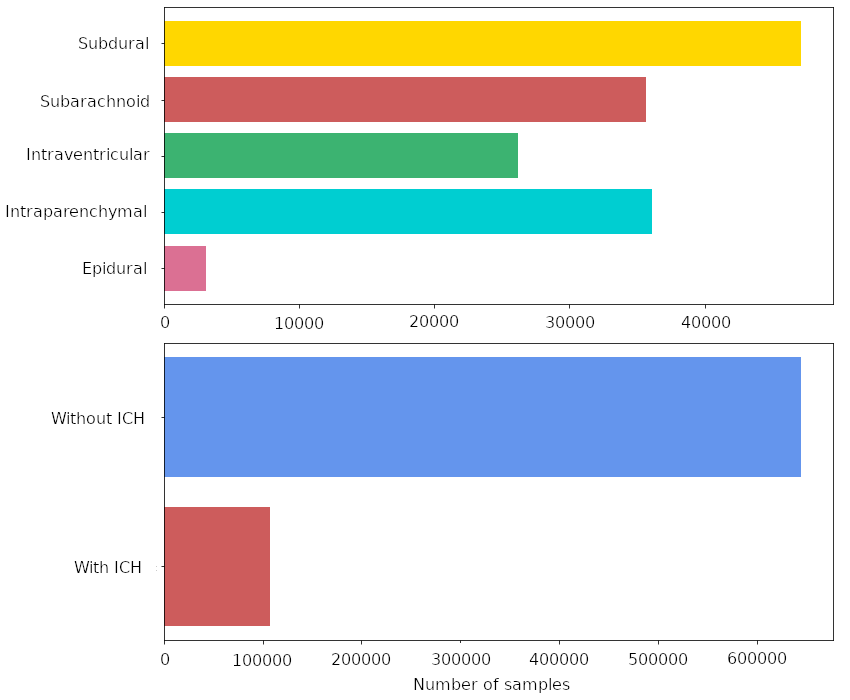
\includegraphics[scale=0.43]{images/num_classes.png}
		\centering
		\caption{In the graph on the top, the numbers of samples representing individual classes in the dataset are plotted. The exact numbers are following: 47\,166 subdural,  35\,675 subarachnoid, 26\,205 intraventricular, 36\,118 intraparenchymal, 3\,145 epidural. In the graph on the bottom, the ratio between samples with ICH and without ICH is shown. The exact numbers are: 644\,874 without ICH and 107\,933 with ICH.}
		\label{fig:types_ratio}
\end{figure}

\section{Experiments}
In order to achieve high accuracy, several experiments were done. These experiments were evaluated using the cross-validation method with three folds (over seven epochs each) to make the result more realistic and reproducible.

For these experiments, the dataset was reduced to 36 527 samples (1078 studies in total) because using the entire dataset would be time-consuming. That is approximately 5\% of the original dataset. The studies were selected so that the ratios between ICH types found in each study were approximately equal (180 studies with epidural ICH, 180 with subdural, ...). After sampling the studies, the labels of the individual samples were still highly imbalanced. Therefore undersampling of the majority class and random oversampling the minority was performed to obtain a balanced dataset.

All the approaches were tried with the use of architectures implemented in Tensorflow Keras with pre-trained weights on the ImageNet dataset. The weighted multi-label log loss with double weight on the \say{any} label was used as the loss function. The input images were augmented using rotation, translation, and zooming during the training phase.

The code was run on Kaggle and Google Colab, and the results were visualized using wandb.ai. The links to the wandb.ai graphs with image preprocessing can be found in the Github repository of this thesis.

Because both, Kaggle and Google Colab provides only a limited amount of time for using GPU, and it takes hours to train the network when the images were being preprocessed at the moment of training, all the images were preprocessed and converted to JPEG format, so during the training, only image augmentation was used.

\subsection{Image preprocessing}
The first approach was to correct HU values in the images and then use a specific window and normalize the values. At first, the values of each slice were shifted by the rescale intercept value corresponding to each image to match the correct values of the Hounsfield scale (in some images, the value of air was 0, so the rescale intercept of value -1000 was applied in order to match the correct value of air which is -1000). Moreover, the CT scanner has a limited range of view, and all the values outside the range are usually set to -2000. These values were set to -1000 to represented the air. Finally, a window of CL 40 and WW 80 was applied, and all slices were normalized between the values 0 and 1.

\begin{figure}[ht]
		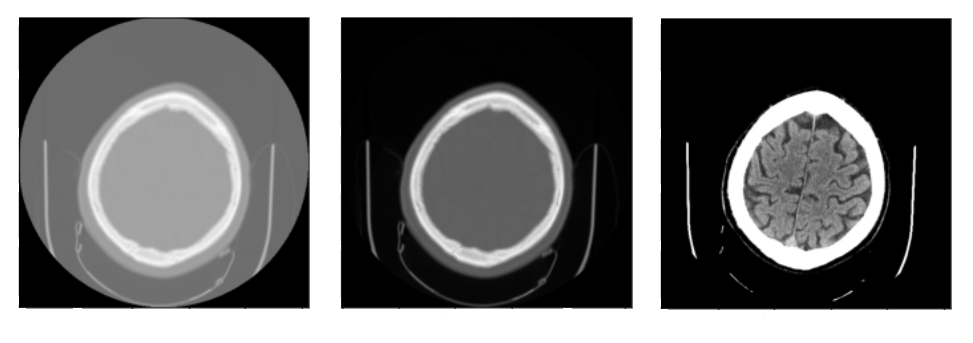
\includegraphics[scale=1.55]{images/correcting_HU.png}
		\centering
		\caption{The process of the first preprocessing approach. On the left, there is a sample without any preprocessing applied. The sample in the middle is after correcting the HU values, and the sample on the right is after using the window with CL 40 and WW 80.}
\end{figure}

A more advanced preprocessing was implemented later. It used the same baseline as in the text above, but it was extended by segmenting the head. The segmentation helped to remove the CT scanner artifacts, so the image contained only the body parts, as shown in Figure \ref{fig:brain_segmentation}. Also, the images varied in-plane resolutions. Hence the resolution was set to 1\,mm\,$\times$\,1\,mm.

\begin{figure}[ht]
		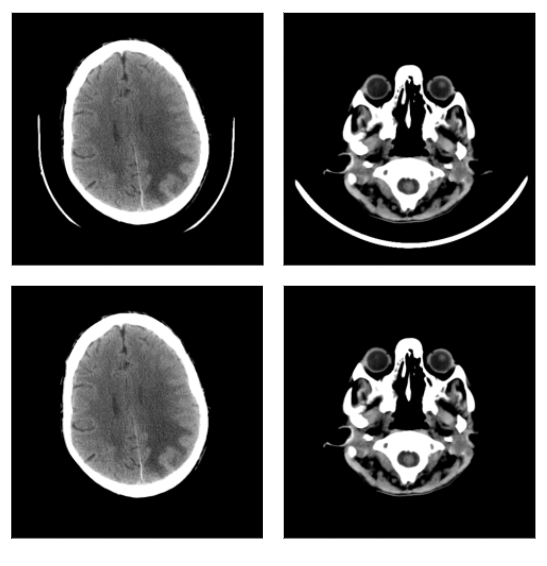
\includegraphics[scale=2.3]{images/image_segmentation.png}
		\centering
		\caption{The top images are before the head segmentation and the bottom after the segmentation.}
		\label{fig:brain_segmentation}
\end{figure}

Other several experiments were tried but not with further improvement of the model's accuracy. One experiment was to put three neighboring slices together that each of the three channels will represent one slice. The intuition was that by providing the additional information from neighboring slices, the model performance would increase, but there was no effect. 

Another experiment was done by changing the model's window. The window used in previous experiments (CL 40, WW 80) is incapable of recognizing some hemorrhages because this window sets all values higher than 80 to white. As was mentioned in Chapter 1, some hemorrhages may occur with higher HU values than 80. Thus if they lie next to the bone or other dense matter, it can be challenging to detect them. Therefore a window with CL 80 and WW 200 was tried, but with this setting the loss get slightly worse with no noticeable effect on the AUC.

Another method used to improve the model's performance was Contrast-limited adaptive histogram equalization (CLAHE), because it is widely used image preprocessing technique used primarily on X-ray images and sometimes CT images. However, this approach was also without further improvement of the models performance. On the contrary, the AUC got worse with the CLAHE.

The last preprocessing method was adding random noise into the image during the augmentation in order to make the model more able to generalize. However, it also did not increase the model's accuracy.

\subsection{Model implementation}
Many experiments were done in order to find the best hyperparameters and architecture. However, before the hyperparameter tuning started, another experiment was done.

Each input image is labeled by five labels representing five types of ICHs, and the last label indicates if any of these types were identified on the given input. Therefore a custom output layer was implemented. This layer takes the maximum of the ICH types predictions and sets this value to the \say{any} label. This approach has improved the validation AUC.

After this improvement, the hyperparameter tuning using the grid search technique was the next step. Different hyperparameters tried were the architectures, batch size, learning rate, learning rate decay rate, and pooling. It shows that the best architectures were DenseNet121 and EfficientNetB0. In the case of the EfficientNet, a learning rate higher than $2\times10^{-5}$ caused instability of the learning, and the model did not convert to the optima. Lower learning rates were stable, but the learning was too slow. Therefore the learning rate of $2\times10^{-5}$ was chosen as the best value. The batch size did not noticeably affect the performance of the network, and using max pooling made the accuracy worse, so the average pooling was chosen.

DenseNet was stable with lower learning rate values than the EfficientNet, so the optimal learning rate was chosen as $10^{-5}$. However, the other hyperparameters had the same impact on both architectures. The performance of these two architectures is shown in Figure \ref{fig:DensexEff}.

\begin{figure}[ht]
		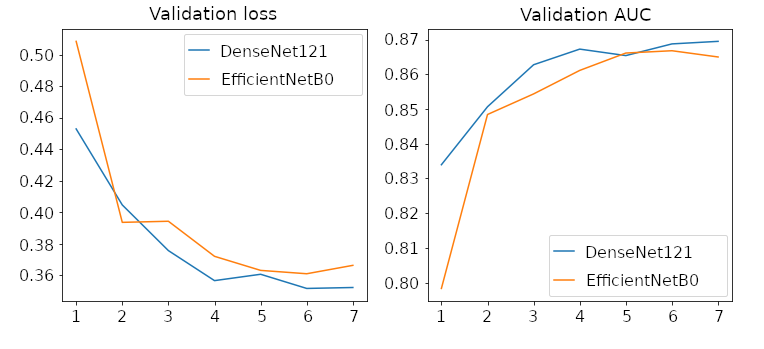
\includegraphics[scale=0.48]{images/DenseNet_x_EfficientNet.png}
		\centering
		\caption{The plots shows the comparison of two architectures that performed best in the experiment phase. The progress of validation loss over seven epochs is shown on the left and the AUC on the right.}
		\label{fig:DensexEff}
\end{figure}

On the other hand, Inception architectures did not work very well, and the ResNets were not as good as DenseNet and EfficientNet.

%\begin{figure}[ht]
%		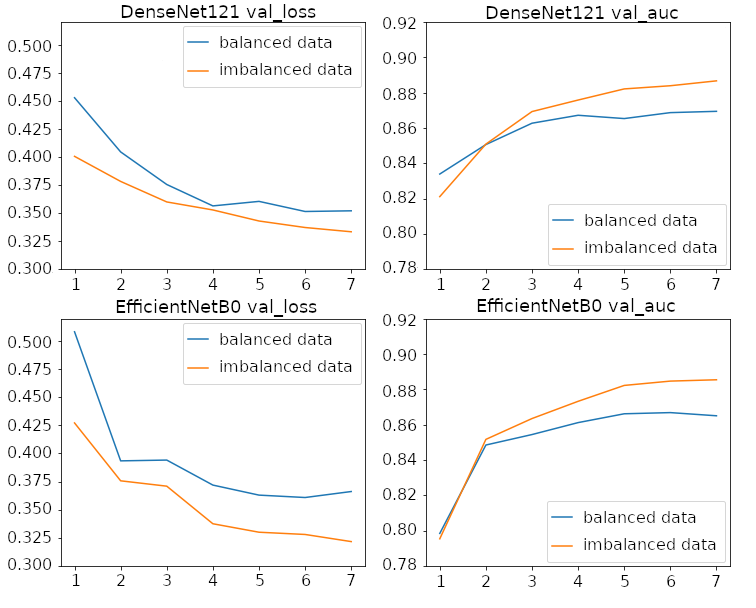
\includegraphics[scale=0.48]{images/balancedXimbalanced.png}
%		\centering
%		\caption{The graphs shows that architectures performed better with imabalanced data than with randomly undersampled and oversampled classes. The $x$ axis refers to number of epochs and $y$ to the weighted multi-label log loss or AUC.}
%		\label{fig:balancedXimbalanced}
%\end{figure}
%
%Another interesting fact is that the experiments showed that the random oversampling caused overfitting of the minority class, and the models performed better on imbalanced datasets.

\section{Final solution and results}
As the final model, two models were chosen. First, an EfficientNetB0 from the Tensorflow Keras library with learning rate $2\times10^{-5}$ using average pooling and batch size 32 and DenseNet121 with the same hyperparameters, but with learning rate $10^{-5}$. These models were chosen because the experiments showed that their setup performed the best. Both architectures were initialized with pre-trained weights on the ImageNet dataset, and they were extended by the last layer, which takes five predictions of the hemorrhage types occurrence and sets the \say{any} label as the max value of these predictions.

Before the training, all input images were preprocessed and saved in JPEG format. The preprocessing approach was chosen based on the results of the experiments. The process was following:
\begin{itemize}
	\item shifting the values by the rescale intercept corresponding to the CT scan;
	\item applying a window of CL 40 and WW 80;
	\item normalizing the values;
	\item segmentation of the brain and avoiding the machine artifacts;
	\item rescaling the image, so the distance between pixels is 1\,mm\,$\times$\,1\,mm;
	\item cropping od padding the image with zeros to get the $224\times224$ shape;
	\item converting from one-channel image to three-channel.
\end{itemize}

Also, the dataset intended for training was divided by studies into a training set and a test set. The test set included 5\% of the studies from the original dataset, and it did not include any of the images used for the experiments. After the separation, the models were trained using a 3-fold cross-validation each over five epochs with balanced dataset obtained by undersampling and oversampling. The weights from all cross-validation folds were saved, and the performance of these models was evaluated independently on the custom test set. Finally, two ensemble models were also evaluated, one model composed of all DenseNets and one of all EfficientNets. However, for further improvement of the performance, test-time augmentation (TTA) was tried. Each image from the test set was augmented five times, the labels were predicted for all of these augmentations, and the average of the predictions was used as the final decision. The performance of the DenseNet and EfficientNet models is shown in Table \ref{tab:DenseNet_performance} and Table \ref{tab:EfficientNet_performance}.

\begin{table}[h]
    \centering
        \begin{tabular}{ |p{3cm}||c|c|c|c|  }
         \hline
         \multicolumn{5}{|c|}{DenseNet121 performance} \\
         \hline
         \hline
         DenseNet121 fold & AUC & ACC & Sensitivity & Specificity\\
         \hline
         Fold 1       & 0.894 & 0.960 & 0.780 & 0.969\\
         Fold 1 TTA   & 0.920 & 0.957 & 0.829 & 0.964\\
         Fold 2       & 0.930 & 0.963 & 0.774 & 0.973\\
         Fold 2 TTA   & 0.952 & 0.958 & 0.829 & 0.966\\
         Fold 3       & 0.915 & 0.959 & 0.771 & 0.970\\
         Fold 3 TTA   & 0.943 & 0.955 & 0.830 & 0.961\\
         Ensemble     & 0.944 & \textbf{0.967} & 0.779 & \textbf{0.978}\\
         Ensemble TTA & \textbf{0.966} & 0.963 & \textbf{0.838} & 0.969\\
         \hline
        \end{tabular}
    \caption{The table shows the performance of three DenseNet121 models trained by 3-fold cross-validation. Each model was evaluated once, and then they were additionally evaluated using TTA. Also, all the models were ensembled, and TTA was also used on the ensembled model.}
    \label{tab:DenseNet_performance}
\end{table}

\begin{table}[h]
    \centering
        \begin{tabular}{ |p{3cm}||c|c|c|c|  }
         \hline
         \multicolumn{5}{|c|}{EfficientNetB0 performance} \\
         \hline
         \hline
         DenseNet121 fold & AUC & ACC & Sensitivity & Specificity\\
         \hline
         Fold 1       & 0.910 & 0.952 & 0.785 & 0.961\\
         Fold 1 TTA   & 0.925 & 0.951 & 0.827 & 0.958\\
         Fold 2       & 0.928 & 0.958 & 0.765 & 0.968\\
         Fold 2 TTA   & 0.946 & 0.955 & 0.810 & 0.963\\
         Fold 3       & 0.913 & 0.951 & 0.792 & 0.960\\
         Fold 3 TTA   & 0.934 & 0.952 & 0.824 & 0.959\\
         Ensemble     & 0.942 & \textbf{0.960} & 0.784 & \textbf{0.970}\\
         Ensemble TTA & \textbf{0.955} & 0.957 & \textbf{0.828} & 0.965\\
         \hline
        \end{tabular}
    \caption{The table shows the performance of three EfficientNetB0 models trained by 3-fold cross-validation. Each model was evaluated once, and then they were additionally evaluated using TTA. Also, all the models were ensembled, and TTA was also used on the ensembled model.}
    \label{tab:EfficientNet_performance}
\end{table}

As shown in the tables, the TTA helped to increase the sensitivity of the model by approximately 5 \%, which is a great improvement. Also, it improved the AUC by 2--3 \% in most cases. On the other hand, it slightly reduced the accuracy (approximately by 0.25 \%) and the specificity (0.5 \%), but the improvement of the sensitivity and AUC is more significant and important, so in the result, the TTA increased the model performance. Also the model ensembling helped especially with increasing the AUC. However, the best model was obtained by using TTA and ensembling the five best models, which were all the DenseNet models and EfficientNet model from the first and third fold. The results are shown in Table  \ref{tab:final_ensemble_performance} and in Table \ref{tab:ref_models_comparison} the final model is compared to the models referenced in Chapter \ref{chap:related_studies}.

\begin{table}[ht]
    \centering
        \begin{tabular}{ |c|c|c|c|  }
         \hline
         \multicolumn{4}{|c|}{DenseNet and EfficientNet ensemble performance} \\
         \hline
         \hline
         AUC & ACC & Sensitivity & Specificity\\
         \hline
         0.967 & 0.963 & 0.840 & 0.970\\
         \hline
        \end{tabular}
    \caption{The table shows the preformance of the final model that uses TTA and consists of all three DenseNet models from the cross-validation and EfficientNet models from fold 1 and 2. }
    \label{tab:final_ensemble_performance}
\end{table}

\begin{table}[ht]
    \centering
        \begin{tabular}{ |p{2.5cm}||c|c|c|c|  }
         \hline
         Model & AUC & ACC & Sensitivity & Specificity\\
         \hline
         \hline
         Ref 1 \cite{DBLP:1710-04934} & --- & 0.818 & 0.886 & ---\\
         Ref 2 \cite{Kuo22737}        & 0.991 & --- & --- & ---\\
         Ref 3 \cite{Chang1609}       & 0.970 & 0.981 & 0.951 & 0.973\\
         Ref 4 \cite{Cho2019}         & --- & --- & 0.979 & 0.988\\
         Final model                  & 0.967 & 0.963 & 0.840 & 0.970\\
         \hline
        \end{tabular}
    \caption{Comparison of the final model with models referenced in the Chapter \ref{chap:related_studies}.}
    \label{tab:ref_models_comparison}
\end{table}

The results are not as excellent as in the referenced literature, but they are promising, and they are a good basis for further research. 

The final model was also used for the classification of the RSNA Intracranial Hemorrhage Detection competition submission dataset. After evaluation, the model achieved a private score of 0.10369. This score was used for the final standings in the leaderboard, and it was computed on more than 99 \% of the test dataset. This result corresponds to the 351.\,place out of 432, which is also not excellent, but the first place has a score of 0.04383, and the differences between places are often in hundredths or thousandth. With further improvement and using more advanced techniques for oversampling the minority data, the sensitivity could increase and so the overall performance.

\section{Discussion}
The two models described above were chosen based on the experiments with image preprocessing and selecting the suitable architecture and hyperparameter tuning. Both models were trained on 95\,\% of the given data using 3-fold cross-validation over five epochs on a balanced dataset, which results in six trained models in total. These models were tested using the remaining 5\,\% of the dataset, improved by using test-time augmentation, and compared with their ensembled versions. The best model was an ensemble of three DenseNet121 and two EfficientNetB0 architectures. The AUC, accuracy, sensitivity, and specificity on the test set were 0.967, 0.963, 0.840, and 0.970, respectively. Additional experiments and research could further improve this result, especially the sensitivity. 

The data was balanced using random undersampling of the majority class and random oversampling of the minority classes, so in the result, the ratios between classes were equal. This approach might cause overfitting of the minority class and low sensitivity as well. More advanced techniques for oversampling that generate synthetic data,  like SMOTE\cite{chawla_bowyer_hall_kegelmeyer_2002} or ADASYN\cite{4633969}, can be used to avoid this problem.

Other experiments could be done using bigger networks, different architectures, or recurrent neural networks, as mentioned in the referenced literature. Also, further improvement may be achieved by using the 3D context in the final classification or using some metadata from the DICOM images.

\setsecnumdepth{part}
\chapter{Conclusion}
This work aimed to research the state-of-the-art techniques used for detection and classification in the medical imaging domain using neural networks, implement own solution that will work on the provided dataset, and finally, compare the results with existing models. 

In the first part of this thesis (Chapter \ref{chap:theoretical_background} and \ref{chap:state_of_the_art}), the theory behind artificial neural networks is described as well as the state-of-art-techniques used in developing and improving such models.

In the practical part of the thesis (Chapter \ref{chap:realization}), many experiments were done, which helped to improve the model. The range of methods used in pre-processing is satisfactory. It has led to a significant improvement of the model, especially using windowing, head segmentation, and rescaling. Furthermore, the model's architecture can still be improved. Introducing the custom layer has improved the model performance as well as the dataset balancing.  Cross-validation and hyperparameter tunning were used to choose the appropriate model. The two best models were selected, and their performance was increased by the test-time augmentation and ensembling. The results were good with slightly lower sensitivity. However, other approaches may help develop a more accurate model, such as more hyperparameter tuning, using more advanced oversampling techniques, modifying the implemented architectures in Keras, trying to incorporate the recurrent neural networks, or developing own custom complex architecture as is done in many research papers mentioned in Chapter \ref{chap:related_studies}. 

\bibliographystyle{iso690}
\bibliography{references}

\setsecnumdepth{all}
\appendix

\chapter{Acronyms}
% \printglossaries
\begin{description}
    \item[AI] Artificial Intelligence
    \item[ANN] Artificial Neural Network
    \item[AUC] Area Under the ROC Curve
    \item[BCE] Binary Cross-Entropy
    \item[CL] Center Level
    \item[CLAHE] Contrast Limited Adaptive Histogram Equalization
    \item[CNN] Convolutional Neural Network
	\item[CT] Computed Tomography
	\item[DRN] Dilated ResNet
	\item[FC] Fully Connected
	\item[FCN] Fully Convolutional Network
	\item[FN] False Negative
	\item[FP] False Positive
	\item[GPU] Graphics Processing Unit
	\item[HU] Hounsfield Unit
	\item[ICH] Intracranial Hemorrhage
	\item[LSTM] Long Short Term Memory
	\item[ML] Machine Learning
	\item[R-CNN] Region with Convolutional Neural Network
	\item[ReLU] Rectified Linear Unit
	\item[RNN] Recurrent Neural Network
	\item[ROC] Reciever Operating Characteristic
	\item[RSNA] Radiological Society of North America
	\item[TN] True Negative
	\item[TP] True Positive
	\item[TTA] Test-Time Augmentation
	\item[WW] Window Width
\end{description}


\chapter{Contents of enclosed SD card}

%change appropriately

\begin{figure}
	\dirtree{%
		.1 README.txt\DTcomment{the file with SD card contents description}.
		.1 src\DTcomment{the directory of .ipynb source codes}.
		.1 thesis\DTcomment{the thesis text and source codes directory}.
		.2 tex\DTcomment{the directory with the \LaTeX{} source codes}.
		.2 thesis.pdf\DTcomment{the thesis text in PDF format}.
	}
\end{figure}

\end{document}
